\documentclass[11pt,openany,a4paper]{article}
\usepackage{amsmath, amsfonts, amssymb, amsthm}
\usepackage{tikz, pgfplots, tkz-euclide,calc}
    \usetikzlibrary{patterns,decorations,shapes.arrows,arrows.meta,angles,quotes}
\usepackage{fancyhdr}
\usepackage{enumerate,enumitem}
\usepackage{cancel}
\usepackage{varwidth}
\usepackage{array}
\usepackage{animate}
\usepackage{xfrac}
\usepackage{multirow,multicol}
\usepackage{hyperref}
\hypersetup{
    colorlinks=true,
    linkcolor=blue,
    filecolor=magenta,      
    urlcolor=cyan,
    pdftitle={Overleaf Example},
    pdfpagemode=FullScreen,
    }
\usepackage{graphicx}
\graphicspath{{C:/Users/teoso/OneDrive/Documents/Asisten Dosen & Lab/Asisten Laboratorium/Alpro 1/PPT/Graphicx/}{C:/Users/teoso/OneDrive/Documents/Tugas Kuliah/Template Math Depart/}}

% TAMBAHKAN PACKAGE SENDIRI KALAU KURANG

\usepackage{geometry}
\geometry{
	left = 20mm,
	right = 20mm,
	top = 30mm,
	bottom = 30mm,
}

\tikzset{
    double arrow/.style={
        double,
        double distance=2pt,
        -{Stealth[length=5pt,width=10pt]}
    }
}


\pagestyle{fancy}
\fancyhead{}
\fancyfoot{}
\fancyhead[r]{}
\fancyhead[l]{\fbox{\large{\textbf{SKPB - ITS}}}}
\renewcommand{\headrulewidth}{0pt}
\renewcommand{\footrulewidth}{0pt}

\newcommand{\R}{\mathbb{R}}
\newcommand{\N}{\mathbb{N}}
\newcommand{\C}{\mathbb{C}}
\newcommand{\Z}{\mathbb{Z}}
\newcommand{\Q}{\mathbb{Q}}
\newcommand{\cis}{\text{cis}}

\begin{document}
\begin{center}
    {\underline{\textbf{\MakeUppercase{Evaluasi Akhir Semester Bersama Ganjil 2024/2025}}}}
\end{center}

\begin{center}
    \begin{tabular}{lcl}
        Mata kuliah/SKS & : & Kalkulus 1 ( SM234101 ) / 3 SKS \\
        Hari, Tanggal   & : & Rabu, 11 Desember 2024          \\
        Waktu           & : & 07.00-08.40 WIB (100 menit)     \\
        Sifat           & : & Tertutup                        \\
        Kelas           & : & 13-19, 103
    \end{tabular}
\end{center}

\noindent\rule{\textwidth}{2.pt}

\setlength{\parindent}{5pt}
\setlength{\parindent}{5pt}
\centering{Tuliskan: Nama, NRP, dan Nomor Kelas pada lembar jawaban Anda.}
\setlength{\parindent}{5pt}
\par \textbf{\small\MakeUppercase{dilarang membawa/menggunakan kalkulator dan alat komunikasi}}
\centering{\textbf{\MakeUppercase{dilarang memberikan/menerima jawaban selama ujian}}}
\par \centering{\textbf{"Setiap tindak kecurangan akan mendapat sanksi akademik."}}
\noindent\rule{\textwidth}{2.pt}

\begin{table}[h]
    \centering
    EAS Mengukur Kemampuan
    \begin{tabular}{|c|m{10.5cm}|c|c|}
        \hline
        CPL & CPMK                                                                                                          & SOAL & BOBOT (\%) \\ \hline
        \multirow{5}{*}{2}
            & CPMK-2 Mampu menentukan kekontinuan fungsi dan                                                                & 1    & 20         \\ \cline{3-4}
            & turunannya                                                                                                    & 2    & 20         \\\cline{2-4}
            & CPMK-3 Mampu menghitung integral melalui teorema fundamental kalkulus                                         & 3    & 20         \\ \cline{2-4}
            & CPMK-4 Mampu mengaplikasikan bentuk peubah kompleks dalam bentuk polar serta mencari akar-akar persamaannya   & 4    & 20         \\ \cline{2-4}
            & CPMK-5 Mampu menerapkan konsep matriks untuk menyelesaikan sistem persamaan linier dan menentukan nilai eigen & 5    & 20         \\ \hline
    \end{tabular}
\end{table}
{\centering\textbf{SOAL}}
% SOAL DI SINI YAA
\begin{enumerate}
    \item
          Suatu persegi panjang memiliki sisi panjang dan lebar yang berubah. Jika sisi panjang bertambah dengan laju 2 cm/menit dan sisi lebar berkurang dengan laju 0.5 cm/menit, dapatkan laju perubahan diagonalnya saat sisi panjangnya mencapai 6 cm dan lebarnya 8 cm.

    \item
          Diberikan fungsi
          $
              f(x) = x^3 - 3x - 1.
          $
          \begin{enumerate}
              \item Tentukan selang dimana fungsi $f(x)$ naik atau turun.
              \item Tentukan titik ekstrem relatif fungsi tersebut.
              \item Tentukan selang kecekungan fungsi $f(x)$ dan titik belok (jika ada).
              \item Sketsa grafiknya.
          \end{enumerate}

    \item
          Hitung integral
          \[
              \int^{4}_{\frac{1}{9}} \frac{6 + 9\sqrt{x}}{\sqrt{x}} \, dx.
          \]

    \item
          Nyatakan bilangan kompleks
          $
              z = \left(\dfrac{-\sqrt{3} + i}{2\cis(15^\circ)}\right)^2
          $
          dalam bentuk $z = a + bi$.

    \item
          Selesaikan sistem persamaan linear berikut:
          \[
              \begin{aligned}
                  3x - z    & = 6,  \\
                  x + y + z & = 15, \\
                  4x + 2z   & = 32,
              \end{aligned}
          \]
          dengan menggunakan metode eliminasi Gauss.
\end{enumerate}
\fancyfoot{\begin{center}
        \rule{0.28\textwidth}{2.pt}$\quad$\textbf{Selamat Mengerjakan}$\quad$\rule{0.28\textwidth}{2.pt}
        \begin{quote}
            \centering
            \textit{``Jujur adalah kunci kesuksesan''}
        \end{quote}
    \end{center}}

\newpage
\fancyhead[L]{\textit{Solution By: \hyperlink{https://github.com/TetewHeroez}{Tetew}}}
\fancyfoot{}
% \fancyfoot[R]{\animategraphics[autoplay,loop,width=0.1\textwidth]{15}{Kuru Kuru Herta/kuru kuru-}{0}{5}}
{\centering\textbf{SOLUSI}}
\renewcommand{\arraystretch}{1.5}
\renewcommand{\headrulewidth}{1pt}
\begin{enumerate}
    \item Perhatikan ilustrasi berikut:
          \begin{center}
              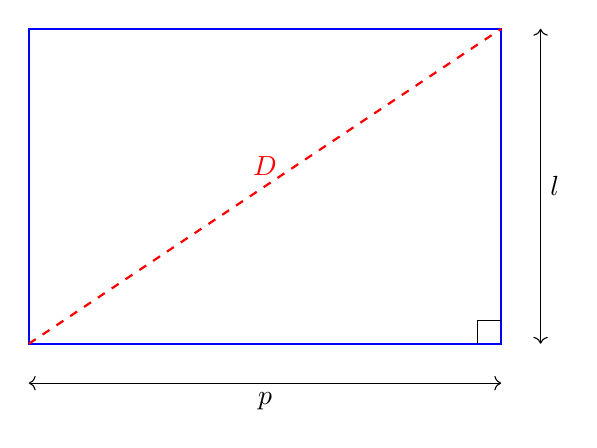
\begin{tikzpicture}[scale=1]
                  % Sisi panjang
                  \draw[thick,blue] (0,0) rectangle (6,4);
                  \draw[<->] (6.5,0) -- (6.5,4) node[midway,right] {$l$};
                  \draw[<->] (0,-0.5) -- (6,-0.5) node[midway,below] {$p$};
                  \draw (5.7,0)|-(6,.3);
                  % Diagonal
                  \draw[thick,dashed,red] (0,0) -- (6,4) node[midway,above] {$D$};
              \end{tikzpicture}
          \end{center}
          Diketahui:
          \[
              \frac{dp}{dt} = 2\ \text{cm/menit}, \quad \frac{dl}{dt} = -0.5\ \text{cm/menit}, \quad p = 6\ \text{cm}, \quad l = 8\ \text{cm}.
          \]
          Dengan menggunakan Teorema Pythagoras, diperoleh hubungan:
          \[
              D^2 = p^2 + l^2.
          \]
          Turunkan terhadap waktu \( t \) (menggunakan diferensiasi implisit):
          \[
              2D \frac{dD}{dt} = 2p \frac{dp}{dt} + 2l \frac{dl}{dt}.
          \]
          Substitusi nilai yang diketahui:
          \[
              2D \frac{dD}{dt} = 2(6)(2) + 2(8)(-0.5).
          \]
          Hitung \( D \) saat \( p = 6 \) cm dan \( l = 8 \) cm:
          \[
              D = \sqrt{6^2 + 8^2} = 10\ \text{cm}.
          \]
          Maka diperoleh:
          \[
              20 \frac{dD}{dt} = 24 - 8 = 16 \iff \frac{dD}{dt} = \frac{4}{5} = 0.8
          \]
          Jadi laju perubahan diagonalnya adalah \( 0.8\ \text{cm/menit} \).

    \item \begin{enumerate}
              \item Uji tanda turunan pertama: $f'(x) = 3x^2 - 3 = 3(x^2 - 1) = 3(x - 1)(x + 1)$.
                    \begin{center}
                        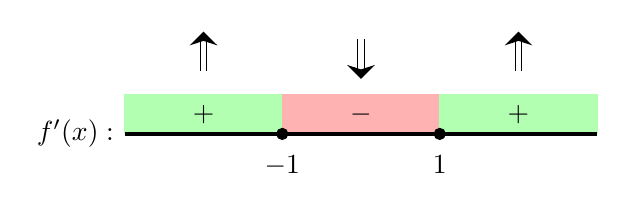
\begin{tikzpicture}[scale=1, baseline]
                            \def\critpoints{-1/black, 1/black}
                            \def\maxint{3}
                            \def\minint{-3}
                            \def\plus{+}

                            %===== Naik/Turun =====
                            % Format: titik_awal / titik_akhir / tanda
                            \foreach \start/\end/\sign in {\minint/-1/+, -1/1/-, 1/\maxint/+} {

                                    % Logika IF untuk menentukan Warna dan Arah Panah
                                    \ifx\sign\plus
                                        \def\mycolor{green!30}  % Warna Hijau
                                        \def\yArrow{0.8}          % Posisi Y awal panah (bawah)
                                        \def\dyArrow{0.5}       % Arah panah (ke atas)
                                    \else
                                        \def\mycolor{red!30}    % Warna Merah
                                        \def\yArrow{1.2}        % Posisi Y awal panah (atas)
                                        \def\dyArrow{-0.5}      % Arah panah (ke bawah)
                                    \fi

                                    \draw[fill=\mycolor, draw=\mycolor] (\start,0) rectangle (\end,0.5) node[midway,black] {$\sign$};

                                    % 2. Gambar Panah
                                    % Titik tengah x dihitung otomatis: (\start + \end) / 2
                                    \draw[double arrow] ({(\start+\end)/2}, \yArrow) -- ++(0, \dyArrow);
                                }
                            %===== GARIS BILANGAN =====
                            \draw[very thick] (\maxint,0) -- (\minint,0) node[left] {$f'(x):$};

                            % loop titik kritis
                            \foreach \x/\c in \critpoints{
                                \draw[fill=\c] (\x,0) circle (2pt);
                                \node[below] at (\x,-0.15) {$\x$}; % label angka
                            }

                        \end{tikzpicture}
                    \end{center}
                    Dari gambar di atas, diperoleh:
                    \begin{itemize}
                        \item Fungsi naik pada interval \( (-\infty, -1) \cup (1, \infty) \).
                        \item Fungsi turun pada interval \( (-1, 1) \).
                    \end{itemize}
              \item Titik kritis diperoleh dari \( f'(x) = 0 \):
                    \[
                        3(x - 1)(x + 1) = 0 \implies x = -1, 1.
                    \]
                    Gunakan uji tanda untuk menentukan jenis titik kritis:
                    \begin{itemize}
                        \item Pada \( x = -1 \), fungsi berubah dari naik ke turun, sehingga \( f(-1) = -1 + 3 - 1 = 1 \) adalah titik maksimum lokal.
                        \item Pada \( x = 1 \), fungsi berubah dari turun ke naik, sehingga \( f(1) = 1 - 3 - 1 = -3 \) adalah titik minimum lokal.
                    \end{itemize}
              \item Uji tanda turunan kedua: \( f''(x) = 6x \).
                    \begin{center}
                        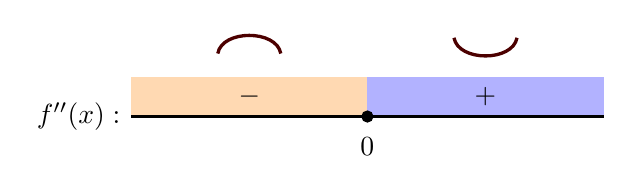
\begin{tikzpicture}[scale=1, baseline]
                            \def\critpoints{0/black}
                            \def\maxint{3}
                            \def\minint{-3}
                            % Pastikan ini ada sebelum loop
                            \def\plus{+}

                            \foreach \start/\end/\sign in {\minint/0/-, 0/\maxint/+} {

                                    % --- LOGIKA ---
                                    \ifx\sign\plus
                                        \def\mycolor{blue!30}
                                        \def\dyArc{1}
                                        \def\direction{right}
                                    \else
                                        \def\mycolor{orange!30}
                                        \def\dyArc{0.8}
                                        \def\direction{left}
                                    \fi

                                    \draw[fill=\mycolor, draw=\mycolor] (\start,0) rectangle (\end,0.5) node[midway,black] {$\sign$};

                                    \draw[very thick, black!70!red]
                                    ({(\start+\end)/2 - 0.4}, \dyArc)
                                    to[bend \direction=80]
                                    ({(\start+\end)/2 + 0.4}, \dyArc);
                                }
                            %===== GARIS BILANGAN =====
                            \draw[very thick] (\maxint,0) -- (\minint,0) node[left] {$f''(x):$};

                            % loop titik kritis
                            \foreach \x/\c in \critpoints {
                                \draw[fill=\c] (\x,0) circle (2pt);   % tick
                                \node[below] at (\x,-0.15) {$\x$}; % label angka
                            }
                        \end{tikzpicture}
                    \end{center}
                    Dari gambar di atas, diperoleh:
                    \begin{itemize}
                        \item Fungsi cekung ke bawah pada interval \( (-\infty, 0) \).
                        \item Fungsi cekung ke atas pada interval \( (0, \infty) \).
                        \item Titik belok pada \( x = 0 \), dengan \( f(0) = -1 \).
                    \end{itemize}
              \item Berdasarkan informasi di atas, sketsa grafiknya adalah sebagai berikut:
                    \begin{center}
                        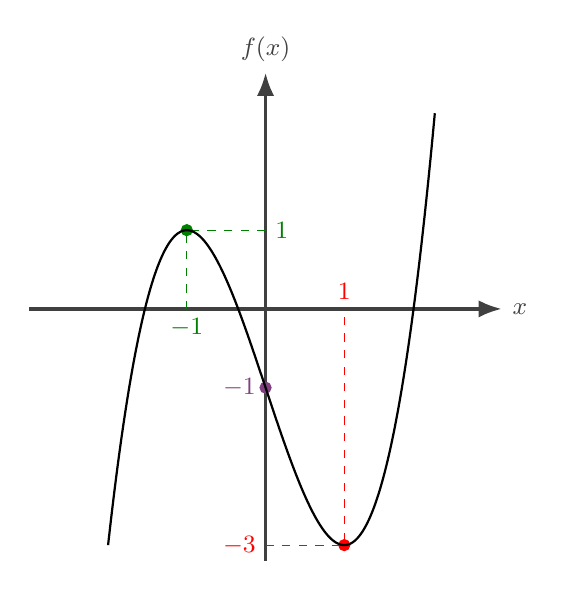
\begin{tikzpicture}[scale=1,every node/.style={font=\small}]
                            % Sumbu x dan y
                            \draw[very thick,-Latex,darkgray] (-3,0) -- (3,0) node[right] {$x$};
                            \draw[very thick,-Latex,darkgray] (0,-3.2) -- (0,3) node[above] {$f(x)$};

                            % Titik ekstrem
                            \draw[dashed,green!50!black] (0,1) node[right] {$1$} -| (-1,0) node[below] {$-1$};
                            \filldraw[green!50!black] (-1,1) circle (2pt);
                            \draw[dashed,red] (0,-3) node[left] {$-3$} -| (1,0) node[above] {$1$};
                            \filldraw[red] (1,-3) circle (2pt);
                            \filldraw[orange!50!blue] (0,-1) circle (2pt) node[left] {$-1$};

                            % Kurva fungsi
                            \draw[thick,domain=-2:2.15,smooth,samples=100] plot (\x, {\x^3 - 3*\x - 1});
                        \end{tikzpicture}
                    \end{center}
          \end{enumerate}
    \item Sederhanakan ekspresi di dalam integral:
          \[
              \frac{6 + 9\sqrt{x}}{\sqrt{x}} = \frac{6}{\sqrt{x}} + \frac{9\sqrt{x}}{\sqrt{x}} = 6x^{-\frac{1}{2}} + 9.
          \]
          Maka integralnya menjadi:
          \begin{align*}
              \int^{4}_{\frac{1}{9}} \frac{6 + 9\sqrt{x}}{\sqrt{x}} \, dx & = \int^{4}_{\frac{1}{9}} 6x^{-\frac{1}{2}} \, dx + \int^{4}_{\frac{1}{9}} 9 \, dx \\
                                                                          & = 6 \left[ 2x^{\frac{1}{2}} \right]^{4}_{\frac{1}{9}} + 9 [x]^{4}_{\frac{1}{9}}   \\
                                                                          & = 12 \left( 2 - \frac{1}{3} \right) + 9 \left( 4 - \frac{1}{9} \right)            \\
                                                                          & = 12 \cdot \frac{5}{3} + 9 \cdot \frac{35}{9} = 20 + 35 = 55.
          \end{align*}
    \item Ubah bilangan kompleks pada pembilang ke bentuk polar:
          \begin{align*}
              r      & = \sqrt{(-\sqrt{3})^2 + 1^2} = \sqrt{4} = 2,               \\
              \theta & = \tan^{-1}\left( \frac{1}{-\sqrt{3}} \right) = 150^\circ.
          \end{align*}
          Sehingga
          \[
              -\sqrt{3} + i = 2\cis(150^\circ).
          \]
          Maka
          \begin{align*}
              z & = \left( \frac{\cancel{2}\cis(150^\circ)}{\cancel{2}\cis(15^\circ)} \right)^2 = \left( \cis(150^\circ-15^\circ) \right)^2 = \left( \cis(135^\circ) \right)^2 = \cis(135^\circ \cdot 2) = \cis(270^\circ) \\
                & = \cos(270^\circ) + i\sin(270^\circ) = (0) + i(-1) = -i.
          \end{align*}
          Jadi $a=0$ dan $b=-1$.

    \item Lakukan OBE pada matriks augmented hingga diperoleh bentuk eselon baris (matriks segitiga atas):
          \begin{align*}
               & \left[
                  \begin{array}{ccc|c}
                      3 & 0 & -1 & 6  \\
                      1 & 1 & 1  & 15 \\
                      4 & 0 & 2  & 32
                  \end{array}
                  \right]
              \begin{array}{c}
                  \xrightarrow{B_1\Leftrightarrow B_2}
              \end{array}
              \left[
                  \begin{array}{ccc|c}
                      1 & 1 & 1  & 15 \\
                      3 & 0 & -1 & 6  \\
                      4 & 0 & 2  & 32
                  \end{array}
                  \right]
              \begin{array}{c}
                  \xrightarrow{B_2- 3B_1} \\
                  \xrightarrow{B_3- 4B_1}
              \end{array}
              \left[
                  \begin{array}{ccc|c}
                      1 & 1  & 1  & 15  \\
                      0 & -3 & -4 & -39 \\
                      0 & -4 & -2 & -28
                  \end{array}
              \right]                                       \\
               & \begin{array}{c}
                     \xrightarrow{B_3-\frac{4}{3}B_2}
                 \end{array}
              \left[
                  \begin{array}{ccc|c}
                      1 & 1  & 1            & 15  \\
                      0 & -3 & -4           & -39 \\
                      0 & 0  & \frac{10}{3} & 24
                  \end{array}
                  \right]
              \begin{array}{c}
                  \xrightarrow{3B_3}
              \end{array}
              \left[
                  \begin{array}{ccc|c}
                      1 & 1  & 1  & 15  \\
                      0 & -3 & -4 & -39 \\
                      0 & 0  & 10 & 72
                  \end{array}
                  \right]
          \end{align*}
          Dari baris ketiga, diperoleh \( z = \frac{72}{10} = \frac{36}{5} \).
          Substitusi ke baris kedua:
          \[
              -3y - 4\left( \frac{36}{5} \right) = -39 \implies -3y - \frac{144}{5} = -39 \implies -3y = -39 + \frac{144}{5} = -\frac{51}{5} \implies y = \frac{17}{5}.
          \]
          Substitusi ke baris pertama:
          \[
              3x + \frac{17}{5} + \frac{36}{5} = 15 \implies 3x + \frac{53}{5} = 15 \implies 3x = 15 - \frac{53}{5} = \frac{22}{5} \implies x = \frac{22}{15}.
          \]
          Jadi, solusi sistem persamaan adalah:
          \[
              x = \frac{22}{15}, \quad y = \frac{17}{5}, \quad z = \frac{36}{5}.
          \]
\end{enumerate}

\newpage
\renewcommand{\arraystretch}{1}
\fancyhead{}
\fancyfoot{}
\fancyhead[r]{}
\fancyhead[l]{\fbox{\large{\textbf{SKPB - ITS}}}}
\renewcommand{\headrulewidth}{0pt}
\renewcommand{\footrulewidth}{0pt}
\begin{center}
    {\underline{\textbf{\MakeUppercase{Evaluasi Akhir Semester Bersama Ganjil 2024/2025}}}}
\end{center}

\begin{center}
    \begin{tabular}{lcl}
        Mata kuliah/SKS & : & Kalkulus 1 ( SM234101 ) / 3 SKS \\
        Hari, Tanggal   & : & Kamis, 12 Desember 2024         \\
        Waktu           & : & 07.00-08.40 WIB (100 menit)     \\
        Sifat           & : & Tertutup                        \\
        Kelas           & : & 5-12, 101
    \end{tabular}
\end{center}

\noindent\rule{\textwidth}{2.pt}

\setlength{\parindent}{5pt}
\setlength{\parindent}{5pt}
\centering{Tuliskan: Nama, NRP, dan Nomor Kelas pada lembar jawaban Anda.}
\setlength{\parindent}{5pt}
\par \textbf{\small\MakeUppercase{dilarang membawa/menggunakan kalkulator dan alat komunikasi}}
\centering{\textbf{\MakeUppercase{dilarang memberikan/menerima jawaban selama ujian}}}
\par \centering{\textbf{"Setiap tindak kecurangan akan mendapat sanksi akademik."}}
\noindent\rule{\textwidth}{2.pt}

\begin{table}[h]
    \centering
    EAS Mengukur Kemampuan
    \begin{tabular}{|c|m{10.5cm}|c|c|}
        \hline
        CPL & CPMK                                                                                                          & SOAL & BOBOT (\%) \\ \hline
        \multirow{5}{*}{2}
            & CPMK-2 Mampu menentukan kekontinuan fungsi dan                                                                & 1    & 20         \\ \cline{3-4}
            & turunannya                                                                                                    & 2    & 20         \\\cline{2-4}
            & CPMK-3 Mampu menghitung integral melalui teorema fundamental kalkulus                                         & 3    & 20         \\ \cline{2-4}
            & CPMK-4 Mampu mengaplikasikan bentuk peubah kompleks dalam bentuk polar serta mencari akar-akar persamaannya   & 4    & 20         \\ \cline{2-4}
            & CPMK-5 Mampu menerapkan konsep matriks untuk menyelesaikan sistem persamaan linier dan menentukan nilai eigen & 5    & 20         \\ \hline
    \end{tabular}
\end{table}
{\centering\textbf{SOAL}}
% SOAL DI SINI YAA
\begin{enumerate}
    \item
          Kerucut terbalik dengan tinggi 18 cm dan jari-jari 9 cm diisi pasir dengan laju 4 cm\(^3\)/menit. Berapa cepat ketinggian pasir dalam kerucut bertambah saat tingginya mencapai 12 cm?

    \item
          Diberikan fungsi
          $\displaystyle
              f(x) = 1 + 3x^2 - 2x^3.
          $
          \begin{enumerate}
              \item Tentukan selang dimana fungsi \( f(x) \) naik atau turun.
              \item Tentukan titik ekstrem relatif fungsi tersebut.
              \item Tentukan selang kecekungan fungsi \( f(x) \) dan titik belok (jika ada).
              \item Sketsa grafiknya.
          \end{enumerate}

    \item
          \begin{enumerate}
              \item Uraikan \( |3x - 3| \) dalam fungsi sepotong-sepotong.
              \item Hitung integral
                    $\displaystyle
                        \int_{0}^{4} |3x - 3| \, dt.
                    $
          \end{enumerate}

    \item
          Nyatakan bilangan kompleks
          $\displaystyle
              z = \frac{i^{19} - 3i^{30}}{1 - 2i}
          $
          dalam bentuk kutub \( z = r\, \cis\,\theta \).

    \item
          Selesaikan sistem persamaan linear berikut:
          \[
              \begin{aligned}
                  3x + 4y + z & = -2, \\
                  3x + 2y + z & = 2,  \\
                  x + y + z   & = 2,
              \end{aligned}
          \]
          dengan menggunakan eliminasi Gauss-Jordan.

\end{enumerate}
\fancyfoot{\begin{center}
        \rule{0.28\textwidth}{2.pt}$\quad$\textbf{Selamat Mengerjakan}$\quad$\rule{0.28\textwidth}{2.pt}
        \begin{quote}
            \centering
            \textit{``Jujur adalah kunci kesuksesan''}
        \end{quote}
    \end{center}}

\newpage
\fancyhead[L]{\textit{Solution By: \hyperlink{https://github.com/TetewHeroez}{Tetew}}}
\fancyfoot{}
% \fancyfoot[R]{\animategraphics[autoplay,loop,width=0.1\textwidth]{15}{Kuru Kuru Herta/kuru kuru-}{0}{5}}
{\centering\textbf{SOLUSI}}
\renewcommand{\arraystretch}{1.5}
\renewcommand{\headrulewidth}{1pt}
\begin{enumerate}
    \item Perhatikan ilustrasi berikut:
          \begin{center}
              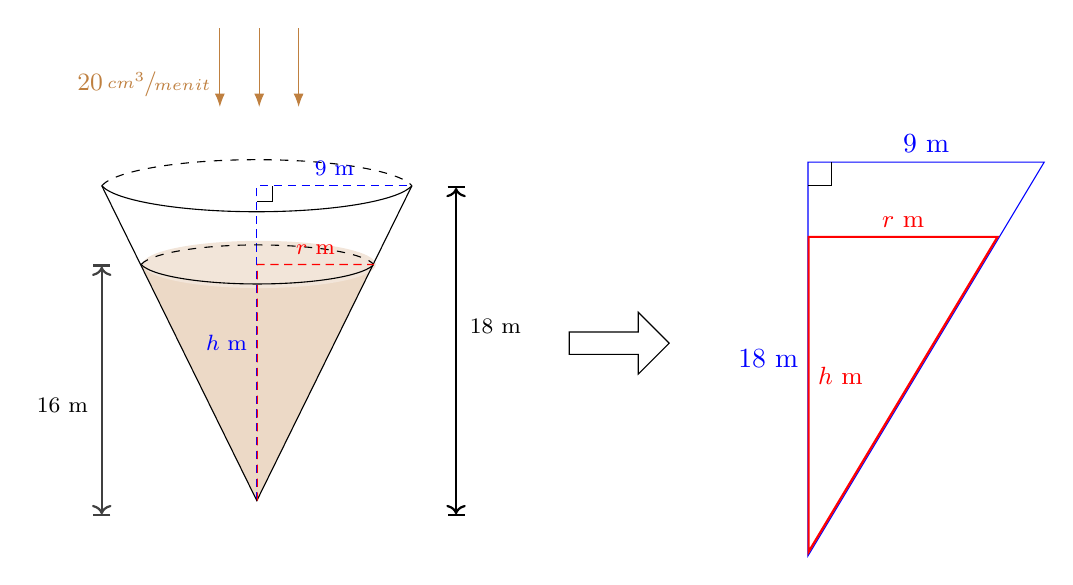
\begin{tikzpicture}
                  \draw[dashed] (0,0) arc (170:10:2cm and 0.4cm)coordinate[pos=0] (a);
                  \draw (0,0) arc (-170:-10:2cm and 0.4cm)coordinate (b);
                  \fill [brown!30!white,opacity=1] (0.5,-1) -- ([yshift=-4cm]$(a)!0.5!(b)$) -- (3.45,-1) -- cycle;
                  \fill [brown!20!white,opacity=1,] (2,-1) circle (1.48cm and 0.3cm);
                  \draw[densely dashed,blue] ([yshift=-4cm]$(a)!0.5!(b)$) -- node[left,font=\footnotesize] {$h$ m}coordinate[pos=0.95] (aa)($(a)!0.5!(b)$)
                  -- node[above,font=\footnotesize] {$9$ m}coordinate[pos=0.1] (bb) (b);
                  \draw (aa) -| (bb);
                  \draw (a) -- ([yshift=-4cm]$(a)!0.5!(b)$) -- (b);
                  \draw[|<->|,thick] (4.5,0)--(4.5,-4.2);
                  \draw[|<->|,thick,darkgray] (0,-1)--(0,-4.2);
                  \coordinate[label=\footnotesize{$18$ m}] () at (5,-2);
                  \coordinate[label=\footnotesize{$16$ m}] () at (-0.5,-3);

                  \draw[dashed] (0.5,-1) arc (170:10:1.5cm and 0.3cm)coordinate[pos=0] (a');
                  \draw (0.5,-1) arc (-170:-10:1.5cm and 0.3cm)coordinate (b');
                  \draw[densely dashed,red] ([yshift=-3cm]$(a')!0.5!(b')$) -- coordinate[pos=0.95] (aa')($(a')!0.5!(b')$)
                  -- node[above,font=\footnotesize] {$r$ m}coordinate[pos=0.1] (bb') (b');

                  \draw [-Latex,brown] (1.5,2) -- (1.5,1) node [above left] {\small{$20\,\sfrac{cm^3}{menit}$}};
                  \draw [-Latex,brown] (2,2) -- (2,1);
                  \draw [-Latex,brown] (2.5,2) -- (2.5,1);

                  \node[fill=white,single arrow, draw] at (6.5,-2) {\color{white}.........};

                  \coordinate (A) at ($(aa)+(10,0.5)$);
                  \coordinate (B) at ($(aa)+(7,0.5)$);
                  \coordinate (C) at ($(aa)+(7,-4.5)$);
                  \draw[blue] (A) -- (B)--+(0,-5)--cycle;
                  \pic [draw, angle radius=3mm] {right angle = A--B--C};
                  \tkzLabelSegment[above,blue](A,B) {$9$ m};
                  \tkzLabelSegment[left,blue](C,B) {$18$ m};

                  \coordinate (A') at ($(aa')+(9.4,0.5)$);
                  \coordinate (B') at ($(aa')+(7,0.5)$);
                  \coordinate (C') at ($(aa)+(7,-3.5)$);
                  \draw[red,thick] (A')--(B')--+(0,-4)--cycle;
                  \tkzLabelSegment[above,red](A',B') {\small$r$ m};
                  \tkzLabelSegment[below right,red](C',B') {\small $h$ m};
              \end{tikzpicture}
          \end{center}
          Menggunakan konsep kesebangunan segitiga, diperoleh persamaan berikut:
          \begin{align*}
              \frac{r}{h} & = \frac{9}{18} = \frac{1}{2} \implies r = \frac{h}{2}.
          \end{align*}
          Sedangkan volume kerucut diberikan oleh rumus
          \begin{align*}
              V & = \frac{1}{3} \pi r^2 h = \frac{1}{3} \pi \left( \frac{h}{2} \right)^2 h = \frac{\pi h^3}{12}.
          \end{align*}
          Turunkan terhadap waktu \( t \):
          \begin{align*}
              \frac{dV}{dt} & = \frac{d}{dt} \left( \frac{\pi h^3}{12} \right) \\
              \frac{dV}{dt} & = \frac{\pi}{12} \cdot 3h^2 \frac{dh}{dt}        \\
              \frac{dV}{dt} & = \frac{\pi h^2}{4} \frac{dh}{dt}                \\
              \frac{dh}{dt} & = \frac{4}{\pi h^2} \frac{dV}{dt}.
          \end{align*}
          Diketahui \( \dfrac{dV}{dt} = 4\ \text{cm}^3/\text{menit} \) dan \( h = 12\ \text{cm} \), maka
          \begin{align*}
              \left.\frac{dh}{dt}\right|_{h=12} & =\frac{4}{\pi h^2} \left.\frac{dV}{dt}\right|_{h=12} = \frac{4}{\pi (12)^2} \cdot 4 = \frac{16}{144\pi} = \frac{1}{9\pi}\ \text{cm/menit}.
          \end{align*}
          Jadi, ketinggian pasir bertambah dengan laju \( \frac{1}{9\pi}\ \text{cm/menit} \) saat tingginya mencapai 12 cm.
    \item \begin{enumerate}
              \item Uji tanda turunan pertama: $f'(x) = 6x - 6x^2 = 6x(1 - x)$.
                    \begin{center}
                        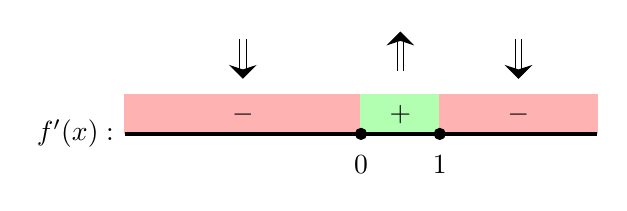
\begin{tikzpicture}[scale=1, baseline]
                            \def\critpoints{0/black, 1/black}
                            \def\maxint{3}
                            \def\minint{-3}
                            \def\plus{+}

                            %===== Naik/Turun =====
                            % Format: titik_awal / titik_akhir / tanda
                            \foreach \start/\end/\sign in {\minint/0/-, 0/1/+, 1/\maxint/-} {

                                    % Logika IF untuk menentukan Warna dan Arah Panah
                                    \ifx\sign\plus
                                        \def\mycolor{green!30}  % Warna Hijau
                                        \def\yArrow{0.8}          % Posisi Y awal panah (bawah)
                                        \def\dyArrow{0.5}       % Arah panah (ke atas)
                                    \else
                                        \def\mycolor{red!30}    % Warna Merah
                                        \def\yArrow{1.2}        % Posisi Y awal panah (atas)
                                        \def\dyArrow{-0.5}      % Arah panah (ke bawah)
                                    \fi

                                    \draw[fill=\mycolor, draw=\mycolor] (\start,0) rectangle (\end,0.5) node[midway,black] {$\sign$};

                                    % 2. Gambar Panah
                                    % Titik tengah x dihitung otomatis: (\start + \end) / 2
                                    \draw[double arrow] ({(\start+\end)/2}, \yArrow) -- ++(0, \dyArrow);
                                }
                            %===== GARIS BILANGAN =====
                            \draw[very thick] (\maxint,0) -- (\minint,0) node[left] {$f'(x):$};

                            % loop titik kritis
                            \foreach \x/\c in \critpoints{
                                \draw[fill=\c] (\x,0) circle (2pt);
                                \node[below] at (\x,-0.15) {$\x$}; % label angka
                            }
                        \end{tikzpicture}
                    \end{center}
                    Dari gambar di atas, diperoleh:
                    \begin{itemize}
                        \item Fungsi naik pada interval \( (0, 1) \).
                        \item Fungsi turun pada interval \( (-\infty, 0) \cup (1, \infty) \).
                    \end{itemize}
              \item Titik kritis diperoleh dari \( f'(x) = 0 \):
                    \[
                        6x(1 - x) = 0 \implies x = 0, 1.
                    \]
                    Gunakan uji tanda untuk menentukan jenis titik kritis:
                    \begin{itemize}
                        \item Pada \( x = 0 \), fungsi berubah dari turun ke naik, sehingga \( f(0) = 1 \) adalah titik minimum lokal.
                        \item Pada \( x = 1 \), fungsi berubah dari naik ke turun, sehingga \( f(1) = 1 + 3 - 2 = 2 \) adalah titik maksimum lokal.
                    \end{itemize}
              \item Uji tanda turunan kedua: \( f''(x) = 6 - 12x \).
                    \begin{center}
                        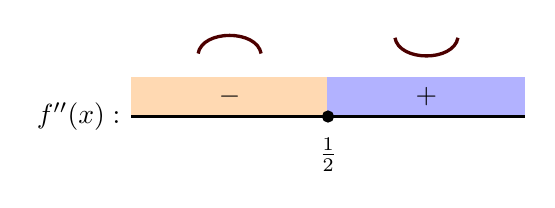
\begin{tikzpicture}[scale=1, baseline]
                            \def\critpoints{0.5/black}
                            \def\maxint{3}
                            \def\minint{-2}
                            % Pastikan ini ada sebelum loop
                            \def\plus{+}

                            \foreach \start/\end/\sign in {\minint/0.5/-, 0.5/\maxint/+} {

                                    % --- LOGIKA ---
                                    \ifx\sign\plus
                                        \def\mycolor{blue!30}
                                        \def\dyArc{1}
                                        \def\direction{right}
                                    \else
                                        \def\mycolor{orange!30}
                                        \def\dyArc{0.8}
                                        \def\direction{left}
                                    \fi

                                    \draw[fill=\mycolor, draw=\mycolor] (\start,0) rectangle (\end,0.5) node[midway,black] {$\sign$};

                                    \draw[very thick, black!70!red]
                                    ({(\start+\end)/2 - 0.4}, \dyArc)
                                    to[bend \direction=80]
                                    ({(\start+\end)/2 + 0.4}, \dyArc);
                                }
                            %===== GARIS BILANGAN =====
                            \draw[very thick] (\maxint,0) -- (\minint,0) node[left] {$f''(x):$};

                            % loop titik kritis
                            \foreach \x/\c in \critpoints {
                                \draw[fill=\c] (\x,0) circle (2pt);   % tick
                                \node[below] at (\x,-0.15) {$\frac{1}{2}$}; % label angka
                            }
                        \end{tikzpicture}
                    \end{center}
                    Dari gambar di atas, diperoleh:
                    \begin{itemize}
                        \item Fungsi cekung ke atas pada interval \( (-\infty, \frac{1}{2}) \).
                        \item Fungsi cekung ke bawah pada interval \( (\frac{1}{2}, \infty) \).
                        \item Titik belok pada \( x = \frac{1}{2} \), dengan \( f\left( \frac{1}{2}\right) = 1 + \frac{3}{4} - \frac{1}{4} = \frac{3}{2} \).
                    \end{itemize}
              \item Berdasarkan informasi di atas, sketsa grafiknya adalah sebagai berikut:
                    \begin{center}
                        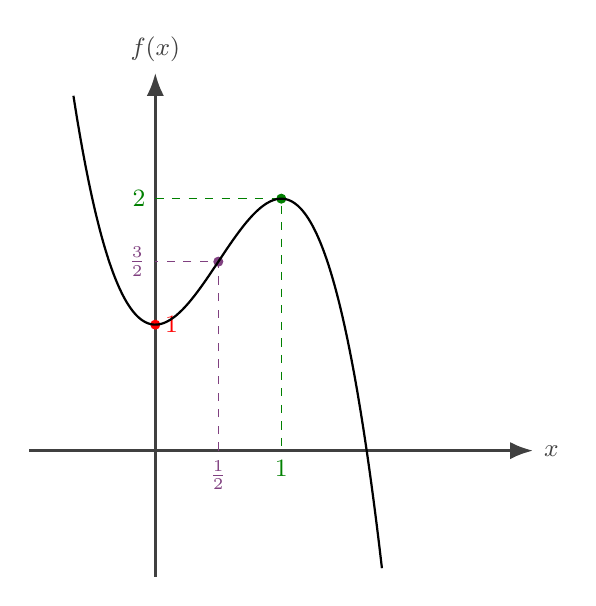
\begin{tikzpicture}[scale=1.6,every node/.style={font=\small}]
                            % Sumbu x dan y
                            \draw[very thick,-Latex,darkgray] (-1,0) -- (3,0) node[right] {$x$};
                            \draw[very thick,-Latex,darkgray] (0,-1) -- (0,3) node[above] {$f(x)$};

                            % Titik ekstrem
                            \draw[dashed,red] (0,1) node[right] {$1$};
                            \filldraw[red] (0,1) circle (1pt);
                            \draw[dashed,green!50!black] (0,2) node[left] {$2$} -| (1,0) node[below] {$1$};
                            \filldraw[green!50!black] (1,2) circle (1pt);
                            \filldraw[orange!50!blue] (0.5,1.5) circle (1pt);
                            \draw[dashed,orange!50!blue] (0.5,0) node[below] {$\frac{1}{2}$} |- (0,1.5) node[left] {$\frac{3}{2}$};

                            % Kurva fungsi
                            \draw[thick,domain=-0.65:1.8,smooth,samples=100] plot (\x, {1 + 3*(\x)^2 - 2*(\x)^3});
                        \end{tikzpicture}
                    \end{center}
          \end{enumerate}
    \item \begin{enumerate}
              \item Uraikan \( |3x - 3| \):
                    \[
                        |3x - 3| =
                        \begin{cases}
                            3x - 3,    & 3x - 3 \geq 0 \\
                            -(3x - 3), & 3x - 3 < 0
                        \end{cases}=\begin{cases}
                            3x - 3,  & x \geq 1 \\
                            -3x + 3, & x < 1
                        \end{cases}
                    \]
              \item Hitung integral:
                    \begin{align*}
                        \int_{0}^{4} |3x - 3| \, dx & = \int_{0}^{1} |3x - 3| \, dx + \int_{1}^{4} |3x - 3| \, dx                                                                                    \\
                                                    & = \int_{0}^{1} (-3x + 3) \, dx + \int_{1}^{4} (3x - 3) \, dx                                                                                   \\
                                                    & = \left[ -\frac{3}{2}x^2 + 3x \right]_{0}^{1} + \left[ \frac{3}{2}x^2 - 3x \right]_{1}^{4}                                                     \\
                                                    & = \left( -\frac{3}{2}(1)^2 + 3(1) - 0 \right) + \left( \left( \frac{3}{2}(4)^2 - 3(4) \right) - \left( \frac{3}{2}(1)^2 - 3(1) \right) \right) \\
                                                    & = \left( -\frac{3}{2} + 3 \right) + \left( (24 - 12) - \left( \frac{3}{2} - 3 \right) \right)                                                  \\
                                                    & = \frac{3}{2} + (12 + \frac{3}{2}) = \frac{3}{2} + \frac{27}{2} = \frac{30}{2} = 15.
                    \end{align*}

          \end{enumerate}
    \item Untuk perpangkatan $i^n$, gunakan pola berikut:
          \begin{align*}
              i^1  = i,   \quad
              i^2  = -1,  \quad
              i^3  = -i,  \quad
              i^4  = 1,   \quad
              i^5  = i,   \quad
              \dots
          \end{align*}
          Sehingga
          \begin{align*}
              i^{19} & = i^{16} \cdot i^3 = 1 \cdot (-i) = -i, \\
              i^{30} & = i^{28} \cdot i^2 = 1 \cdot (-1) = -1.
          \end{align*}
          Maka
          \begin{align*}
              z & = \frac{-i - 3(-1)}{1 - 2i} = \frac{-i + 3}{1 - 2i} = \frac{3 - i}{1 - 2i} \cdot \frac{1 + 2i}{1 + 2i} = \frac{(3 - i)(1 + 2i)}{(1 - 2i)(1 + 2i)} \\
                & = \frac{3 + 6i - i - 2i^2}{1 + 4} = \frac{5 + 5i}{5} = 1 + i.
          \end{align*}
          Ubah ke bentuk kutub:
          \begin{align*}
              r      & = |z| = \sqrt{1^2 + 1^2} = \sqrt{2},              \\
              \theta & = \tan^{-1}\left( \frac{1}{1} \right) = 45^\circ.
          \end{align*}
          Jadi, bentuk kutubnya adalah
          $
              z = \sqrt{2}\, \cis\, 45^\circ.
          $
    \item Lakukan OBE pada matriks augmented hingga diperoleh bentuk eselon baris tereduksi:
          \begin{align*}
               & \left[
                  \begin{array}{ccc|c}
                      3 & 4 & 1 & -2 \\
                      3 & 2 & 1 & 2  \\
                      1 & 1 & 1 & 2
                  \end{array}
                  \right]
              \begin{array}{c}
                  \xrightarrow{B_1\Leftrightarrow B_3}
              \end{array}
              \left[
                  \begin{array}{ccc|c}
                      1 & 1 & 1 & 2  \\
                      3 & 2 & 1 & 2  \\
                      3 & 4 & 1 & -2
                  \end{array}
                  \right]
              \begin{array}{c}
                  \xrightarrow{B_2 - 3B_1} \\
                  \xrightarrow{B_3 - 3B_1}
              \end{array}
              \left[
                  \begin{array}{ccc|c}
                      1 & 1  & 1  & 2  \\
                      0 & -1 & -2 & -4 \\
                      0 & 1  & -2 & -8
                  \end{array}
              \right]                   \\
               & \begin{array}{c}
                     \xrightarrow{B_3 + B_2}
                 \end{array}
              \left[
                  \begin{array}{ccc|c}
                      1 & 1  & 1  & 2   \\
                      0 & -1 & -2 & -4  \\
                      0 & 0  & -4 & -12
                  \end{array}
                  \right]
              \begin{array}{c}
                  \xrightarrow{-\frac{1}{4}B_3}
                  \xrightarrow{-B_2}
              \end{array}
              \left[
                  \begin{array}{ccc|c}
                      1 & 1 & 1 & 2 \\
                      0 & 1 & 2 & 4 \\
                      0 & 0 & 1 & 3
                  \end{array}
                  \right]
              \begin{array}{c}
                  \xrightarrow{B_1 - B_3} \\
                  \xrightarrow{B_2 - 2B_3}
              \end{array}
              \left[
                  \begin{array}{ccc|c}
                      1 & 1 & 0 & -1 \\
                      0 & 1 & 0 & -2 \\
                      0 & 0 & 1 & 3
                  \end{array}
              \right]                   \\
               & \begin{array}{c}
                     \xrightarrow{B_1 - B_2}
                 \end{array}
              \left[
                  \begin{array}{ccc|c}
                      1 & 0 & 0 & 1  \\
                      0 & 1 & 0 & -2 \\
                      0 & 0 & 1 & 3
                  \end{array}
                  \right]\implies
              \begin{matrix}
                  x & = & 1,  \\
                  y & = & -2, \\
                  z & = & 3.
              \end{matrix}
          \end{align*}
\end{enumerate}

\newpage
\renewcommand{\arraystretch}{1}
\fancyhead{}
\fancyfoot{}
\fancyhead[r]{}
\fancyhead[l]{\fbox{\large{\textbf{SKPB - ITS}}}}
\renewcommand{\headrulewidth}{0pt}
\renewcommand{\footrulewidth}{0pt}
\begin{center}
    {\underline{\textbf{\MakeUppercase{Evaluasi Akhir Semester Bersama Ganjil 2024/2025}}}}
\end{center}

\begin{center}
    \begin{tabular}{lcl}
        Mata kuliah/SKS & : & Kalkulus 1 ( SM234101 ) / 3 SKS \\
        Hari, Tanggal   & : & Kamis, 12 Desember 2024         \\
        Waktu           & : & 09.00-10.40 WIB (100 menit)     \\
        Sifat           & : & Tertutup                        \\
        Kelas           & : & 47-59, 111
    \end{tabular}
\end{center}

\noindent\rule{\textwidth}{2.pt}

\setlength{\parindent}{5pt}
\setlength{\parindent}{5pt}
\centering{Tuliskan: Nama, NRP, dan Nomor Kelas pada lembar jawaban Anda.}
\setlength{\parindent}{5pt}
\par \textbf{\small\MakeUppercase{dilarang membawa/menggunakan kalkulator dan alat komunikasi}}
\centering{\textbf{\MakeUppercase{dilarang memberikan/menerima jawaban selama ujian}}}
\par \centering{\textbf{"Setiap tindak kecurangan akan mendapat sanksi akademik."}}
\noindent\rule{\textwidth}{2.pt}

\begin{table}[h]
    \centering
    EAS Mengukur Kemampuan
    \begin{tabular}{|c|m{10.5cm}|c|c|}
        \hline
        CPL & CPMK                                                                                                          & SOAL & BOBOT (\%) \\ \hline
        \multirow{5}{*}{2}
            & CPMK-2 Mampu menentukan kekontinuan fungsi dan                                                                & 1    & 20         \\ \cline{3-4}
            & turunannya                                                                                                    & 2    & 20         \\\cline{2-4}
            & CPMK-3 Mampu menghitung integral melalui teorema fundamental kalkulus                                         & 3    & 20         \\ \cline{2-4}
            & CPMK-4 Mampu mengaplikasikan bentuk peubah kompleks dalam bentuk polar serta mencari akar-akar persamaannya   & 4    & 20         \\ \cline{2-4}
            & CPMK-5 Mampu menerapkan konsep matriks untuk menyelesaikan sistem persamaan linier dan menentukan nilai eigen & 5    & 20         \\ \hline
    \end{tabular}
\end{table}
{\centering\textbf{SOAL}}
% SOAL DI SINI YAA
\begin{enumerate}
    \item
          Suatu pasir dituangkan dari wadah tertentu sedemikian rupa sehingga tumpukan pasir tersebut membentuk kerucut dengan ketinggiannya sama dengan \( \dfrac{1}{3} \) dari diameternya setiap saat. Jika ketinggiannya bertambah dengan laju 4 m/menit, dapatkan laju pertambahan volume tumpukan pasir tersebut saat ketinggiannya mencapai 10 meter.

    \item
          Diberikan fungsi
          $
              f(x) = 1 + (1 - 2x)^3.
          $
          \begin{enumerate}
              \item Tentukan selang dimana fungsi \( f(x) \) naik atau turun.
              \item Tentukan titik ekstrem relatif fungsi tersebut.
              \item Tentukan selang kecekungan fungsi \( f(x) \) dan titik belok (jika ada).
              \item Sketsa grafiknya.
          \end{enumerate}

    \item
          Misalkan
          $\displaystyle
              F(x) = \int_{0}^{x} \frac{t + 1}{t^2 + 1}\, dt,
          $ untuk $-\infty < x < \infty.
          $
          \begin{enumerate}
              \item Dapatkan selang dimana fungsi \( F(x) \) naik atau turun.
              \item Dapatkan selang kecekungan fungsi \( F(x) \).
          \end{enumerate}

    \item
          Dapatkan semua bilangan kompleks \( z \) yang memenuhi
          $
              z^3 = \sqrt{3} + i.
          $

    \item
          Selesaikan sistem persamaan linear berikut:
          \[
              \begin{aligned}
                  2x + 4y + z  & = 7, \\
                  3x + 2y + 2z & = 1, \\
                  x + y + z    & = 0,
              \end{aligned}
          \]
          dengan menggunakan metode invers.

\end{enumerate}
\fancyfoot{\begin{center}
        \rule{0.28\textwidth}{2.pt}$\quad$\textbf{Selamat Mengerjakan}$\quad$\rule{0.28\textwidth}{2.pt}
        \begin{quote}
            \centering
            \textit{``Jujur adalah kunci kesuksesan''}
        \end{quote}
    \end{center}}

\newpage
\fancyhead[L]{\textit{Solution By: \hyperlink{https://github.com/TetewHeroez}{Tetew}}}
\fancyfoot{}
% \fancyfoot[R]{\animategraphics[autoplay,loop,width=0.1\textwidth]{15}{Kuru Kuru Herta/kuru kuru-}{0}{5}}
{\centering\textbf{SOLUSI}}
\renewcommand{\arraystretch}{1.5}
\renewcommand{\headrulewidth}{1pt}
\begin{enumerate}
    \item Perhatikan ilustrasi berikut:
          \begin{center}
              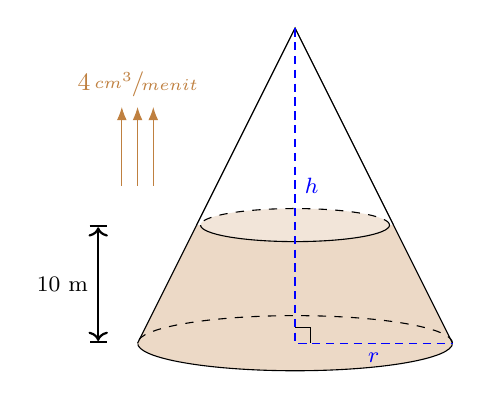
\begin{tikzpicture}
                  \draw[fill=brown!30!white] (-2,0) -- (0,4) -- (2,0);
                  \draw[fill=white] (-1.25,1.5) -- (0,4) -- (1.25,1.5);
                  \begin{scope}
                      \clip (-2,0) rectangle (2,1cm);
                      \draw[dashed] (0,0) circle(2cm and 0.35cm);
                  \end{scope}
                  \begin{scope}
                      \clip (-2,0) rectangle (2,-0.4cm);
                      \draw[fill=brown!30!white] (0,0) circle(2cm and 0.35cm);
                  \end{scope}
                  \begin{scope}
                      \clip (-2,1.5) rectangle (2,2cm);
                      \draw[dashed,fill=brown!20!white] (0,1.5) circle(1.2cm and 0.21cm);
                  \end{scope}
                  \begin{scope}
                      \clip (-2,1.5) rectangle (2,-0.4cm);
                      \draw[fill=brown!20!white] (0,1.5) circle(1.2cm and 0.21cm);
                  \end{scope}
                  \draw[densely dashed,blue] (0,4) -- node[right,font=\footnotesize] {$h$}coordinate[pos=0.95] (aa)(0,0)
                  -- node[below,font=\footnotesize] {$r$}coordinate[pos=0.1] (bb) (2,0);
                  \draw (aa) -| (bb);

                  \draw [-Latex,brown] (-2,2) -- (-2,3) node [above] {\small{$4\,\sfrac{cm^3}{menit}$}};
                  \draw [-Latex,brown] (-2.2,2) -- (-2.2,3);
                  \draw [-Latex,brown] (-1.8,2) -- (-1.8,3);

                  \draw[|<->|,thick] (-2.5,0)--(-2.5,1.5) node[midway,left,font=\footnotesize] {$10$ m};
              \end{tikzpicture}
          \end{center}
          Selanjutnya berdasarkan informasi pada soal, diperoleh bahwa \( h = \dfrac{1}{3} \cdot 2r \implies r = \dfrac{3h}{2} \).
          Volume kerucut diberikan oleh rumus
          \begin{align*}
              V & = \frac{1}{3} \pi r^2 h = \frac{1}{3} \pi \left( \frac{3h}{2} \right)^2 h = \frac{3\pi h^3}{4}.
          \end{align*}
          Turunkan terhadap waktu \( t \):
          \begin{align*}
              \frac{dV}{dt} & = \frac{d}{dt} \left( \frac{3\pi h^3}{4} \right) \\
              \frac{dV}{dt} & = \frac{3\pi}{4} \cdot 3h^2 \frac{dh}{dt}        \\
              \frac{dV}{dt} & = \frac{9\pi h^2}{4} \frac{dh}{dt}               \\
              \frac{dh}{dt} & = \frac{4}{9\pi h^2} \frac{dV}{dt}.
          \end{align*}
          Diketahui \( \dfrac{dh}{dt} = 4\ \text{m/menit} \) dan \( h = 10\ \text{m} \), maka
          \begin{align*}
              \left.\frac{dV}{dt}\right|_{h=10} & =\frac{9\pi h^2}{4} \left.\frac{dh}{dt}\right|_{h=10} = \frac{9\pi (10)^2}{4} \cdot 4 = 900\pi\ \text{m}^3/\text{menit}.
          \end{align*}
          Jadi, volume tumpukan pasir bertambah dengan laju \( 900\pi\ \text{m}^3/\text{menit} \) saat ketinggiannya mencapai 10 meter.
    \item \begin{enumerate}
              \item Uji tanda turunan pertama: $f'(x) = -6(1 - 2x)^2$.
                    \begin{center}
                        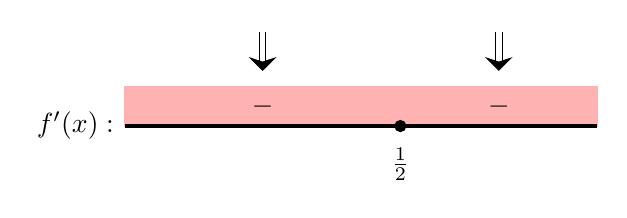
\begin{tikzpicture}[scale=1, baseline]
                            \def\critpoints{0.5/black}
                            \def\maxint{3}
                            \def\minint{-3}
                            \def\plus{+}

                            %===== Naik/Turun =====
                            % Format: titik_awal / titik_akhir / tanda
                            \foreach \start/\end/\sign in {\minint/0.5/-,0.5/\maxint/-} {

                                    % Logika IF untuk menentukan Warna dan Arah Panah
                                    \ifx\sign\plus
                                        \def\mycolor{green!30}  % Warna Hijau
                                        \def\yArrow{0.8}          % Posisi Y awal panah (bawah)
                                        \def\dyArrow{0.5}       % Arah panah (ke atas)
                                    \else
                                        \def\mycolor{red!30}    % Warna Merah
                                        \def\yArrow{1.2}        % Posisi Y awal panah (atas)
                                        \def\dyArrow{-0.5}      % Arah panah (ke bawah)
                                    \fi

                                    \draw[fill=\mycolor, draw=\mycolor] (\start,0) rectangle (\end,0.5) node[midway,black] {$\sign$};

                                    % 2. Gambar Panah
                                    % Titik tengah x dihitung otomatis: (\start + \end) / 2
                                    \draw[double arrow] ({(\start+\end)/2}, \yArrow) -- ++(0, \dyArrow);
                                }
                            %===== GARIS BILANGAN =====
                            \draw[very thick] (\maxint,0) -- (\minint,0) node[left] {$f'(x):$};

                            % loop titik kritis
                            \foreach \x/\c in \critpoints{
                                \draw[fill=\c] (\x,0) circle (2pt);
                                \node[below] at (\x,-0.15) {$\frac{1}{2}$}; % label angka
                            }
                        \end{tikzpicture}
                    \end{center}
                    Dari gambar di atas, diperoleh:
                    \begin{itemize}
                        \item Fungsi turun pada interval \( \left(-\infty,\dfrac{1}{2}\right) \cup \left(\dfrac{1}{2},\infty\right) \).
                        \item Fungsi tidak pernah naik.
                    \end{itemize}
              \item Titik kritis diperoleh dari \( f'(x) = 0 \):
                    \[
                        -6(1 - 2x)^2 = 0 \implies x = \frac{1}{2}.
                    \]
                    Gunakan uji tanda untuk menentukan jenis titik kritis:
                    \begin{itemize}
                        \item Pada \( x = \frac{1}{2} \), fungsi tetap turun di kedua sisi, sehingga tidak ada titik ekstrem relatif (baik maksimum maupun minimum).
                    \end{itemize}
              \item Uji tanda turunan kedua: \( f''(x) = 24(1 - 2x) \).
                    \begin{center}
                        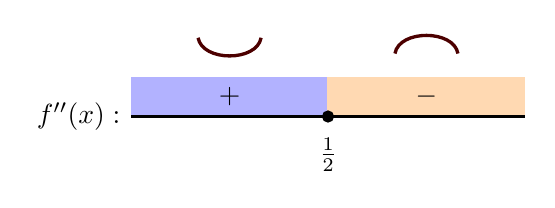
\begin{tikzpicture}[scale=1, baseline]
                            \def\critpoints{0.5/black}
                            \def\maxint{3}
                            \def\minint{-2}
                            % Pastikan ini ada sebelum loop
                            \def\plus{+}

                            \foreach \start/\end/\sign in {\minint/0.5/+, 0.5/\maxint/-} {

                                    % --- LOGIKA ---
                                    \ifx\sign\plus
                                        \def\mycolor{blue!30}
                                        \def\dyArc{1}
                                        \def\direction{right}
                                    \else
                                        \def\mycolor{orange!30}
                                        \def\dyArc{0.8}
                                        \def\direction{left}
                                    \fi

                                    \draw[fill=\mycolor, draw=\mycolor] (\start,0) rectangle (\end,0.5) node[midway,black] {$\sign$};

                                    \draw[very thick, black!70!red]
                                    ({(\start+\end)/2 - 0.4}, \dyArc)
                                    to[bend \direction=80]
                                    ({(\start+\end)/2 + 0.4}, \dyArc);
                                }
                            %===== GARIS BILANGAN =====
                            \draw[very thick] (\maxint,0) -- (\minint,0) node[left] {$f''(x):$};

                            % loop titik kritis
                            \foreach \x/\c in \critpoints {
                                \draw[fill=\c] (\x,0) circle (2pt);   % tick
                                \node[below] at (\x,-0.15) {$\frac{1}{2}$}; % label angka
                            }
                        \end{tikzpicture}
                    \end{center}
                    Dari gambar di atas, diperoleh:
                    \begin{itemize}
                        \item Fungsi cekung ke atas pada interval \( (-\infty, \frac{1}{2}) \).
                        \item Fungsi cekung ke bawah pada interval \( (\frac{1}{2}, \infty) \).
                        \item Titik belok pada \( x = \frac{1}{2} \), dengan \( f\left( \frac{1}{2}\right) = 1 + (1 - 1)^3 = 1 \).
                    \end{itemize}
              \item Tambahkan beberapa informasi seperti titik potong terhadap sumbu $x$ dan $y$, yaitu:
                    \begin{align*}
                        f(x) & = 0 \implies 1 + (1 - 2x)^3 = 0 \implies (1 - 2x)^3 = -1 \implies 1 - 2x = -1 \implies x = 1, \\
                        f(0) & = 1 + (1 - 0)^3 = 1 + 1 = 2.
                    \end{align*}
                    \begin{center}
                        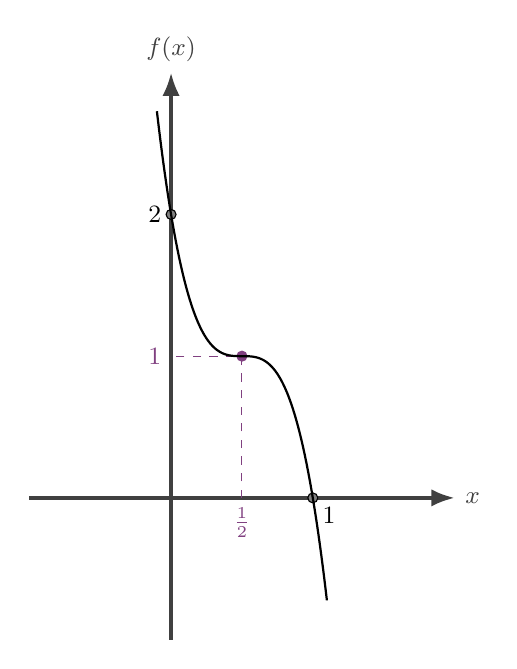
\begin{tikzpicture}[scale=1.8,every node/.style={font=\small}]
                            % Sumbu x dan y
                            \draw[very thick,-Latex,darkgray] (-1,0) -- (2,0) node[right] {$x$};
                            \draw[very thick,-Latex,darkgray] (0,-1) -- (0,3) node[above] {$f(x)$};

                            % Titik ekstrem
                            \filldraw[orange!50!blue] (0.5,1) circle (1pt);
                            \draw[dashed,orange!50!blue] (0.5,0) node[below] {$\frac{1}{2}$} |- (0,1) node[left] {$1$};
                            \draw[fill=gray] (0,2) circle (1pt) node[left] {$2$};
                            \draw[fill=gray] (1,0) circle (1pt) node[below right] {$1$};

                            % Kurva fungsi
                            \draw[thick,domain=-0.1:1.1,smooth,samples=100] plot (\x, {1 + (1 - 2*(\x))^3});
                        \end{tikzpicture}
                    \end{center}
          \end{enumerate}
    \item \begin{enumerate}
              \item Untuk menentukan selang naik/turun, maka diperlukan informasi mengenai tanda dari \( F'(x) \).
                    Berdasarkan Teorema Fundamental Kalkulus, diperoleh
                    \[
                        F'(x) = \frac{d}{dx} \left( \int_{0}^{x} \frac{t + 1}{t^2 + 1}\, dt \right) = \frac{x + 1}{x^2 + 1}.
                    \]
                    Selanjutnya, tinjau tanda \( F'(x) \):
                    \begin{center}
                        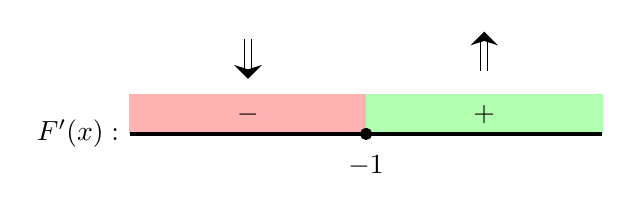
\begin{tikzpicture}[scale=1, baseline]
                            \def\critpoints{-1/black}
                            \def\maxint{2}
                            \def\minint{-4}
                            \def\plus{+}

                            %===== Naik/Turun =====
                            % Format: titik_awal / titik_akhir / tanda
                            \foreach \start/\end/\sign in {\minint/-1/-, -1/\maxint/+} {

                                    % Logika IF untuk menentukan Warna dan Arah Panah
                                    \ifx\sign\plus
                                        \def\mycolor{green!30}  % Warna Hijau
                                        \def\yArrow{0.8}          % Posisi Y awal panah (bawah)
                                        \def\dyArrow{0.5}       % Arah panah (ke atas)
                                    \else
                                        \def\mycolor{red!30}    % Warna Merah
                                        \def\yArrow{1.2}        % Posisi Y awal panah (atas)
                                        \def\dyArrow{-0.5}      % Arah panah (ke bawah)
                                    \fi

                                    \draw[fill=\mycolor, draw=\mycolor] (\start,0) rectangle (\end,0.5) node[midway,black] {$\sign$};

                                    % 2. Gambar Panah
                                    % Titik tengah x dihitung otomatis: (\start + \end) / 2
                                    \draw[double arrow] ({(\start+\end)/2}, \yArrow) -- ++(0, \dyArrow);
                                }
                            %===== GARIS BILANGAN =====
                            \draw[very thick] (\maxint,0) -- (\minint,0) node[left] {$F'(x):$};

                            % loop titik kritis
                            \foreach \x/\c in \critpoints{
                                \draw[fill=\c] (\x,0) circle (2pt);
                                \node[below] at (\x,-0.15) {$-1$}; % label angka
                            }
                        \end{tikzpicture}
                    \end{center}
                    Dari gambar di atas, diperoleh:
                    \begin{itemize}
                        \item Fungsi turun pada interval \( (-\infty,-1) \).
                        \item Fungsi naik pada interval \( (-1,\infty) \).
                    \end{itemize}
              \item Untuk menentukan selang kecekungan, maka diperlukan informasi mengenai tanda dari \( F''(x) \).
                    Turunkan \( F'(x) \):
                    \begin{align*}
                        F''(x) & = \frac{d}{dx} \left( \frac{x + 1}{x^2 + 1} \right) = \frac{(1)(x^2 + 1) - (x + 1)(2x)}{(x^2 + 1)^2}                 \\
                               & = \frac{x^2 + 1 - 2x^2 - 2x}{(x^2 + 1)^2} = \frac{-x^2 - 2x + 1}{(x^2 + 1)^2} = \frac{-(x^2 + 2x - 1)}{(x^2 + 1)^2}.
                    \end{align*}
                    Selanjutnya, tinjau tanda \( F''(x) \):
                    \begin{center}
                        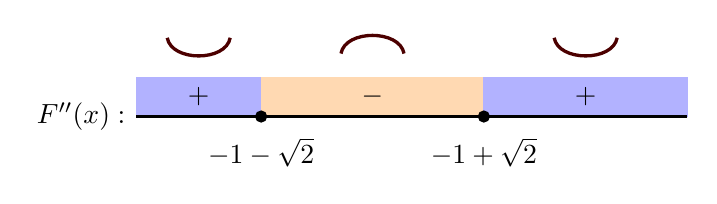
\begin{tikzpicture}[scale=1, baseline]
                            \def\critpoints{-1-sqrt(2)/black/-, -1+sqrt(2)/black/+}
                            \def\maxint{3}
                            \def\minint{-4}
                            \def\plus{+}

                            %===== Naik/Turun =====
                            % Format: titik_awal / titik_akhir / tanda
                            \foreach \start/\end/\sign in {\minint/{-1 - sqrt(2)}/+, {-1 - sqrt(2)}/{-1 + sqrt(2)}/-, {-1 + sqrt(2)}/\maxint/+} {

                            % Logika IF untuk menentukan Warna dan Arah Panah
                            \ifx\sign\plus
                                \def\mycolor{blue!30}
                                \def\dyArc{1}
                                \def\direction{right}
                            \else
                                \def\mycolor{orange!30}
                                \def\dyArc{0.8}
                                \def\direction{left}
                            \fi

                            \draw[fill=\mycolor, draw=\mycolor] ({\start},0) rectangle ({\end},0.5) node[midway,black] {$\sign$};

                            \draw[very thick, black!70!red]
                            ({(\start+\end)/2 - 0.4}, \dyArc)
                            to[bend \direction=80]
                            ({(\start+\end)/2 + 0.4}, \dyArc);
                            }
                            %===== GARIS BILANGAN =====
                            \draw[very thick] (\maxint,0) -- (\minint,0) node[left] {$F''(x):$};
                            % loop titik kritis
                            \foreach \x/\c/\s in \critpoints{
                                \draw[fill=\c] ({\x},0) circle (2pt);
                                \node[below] at ({\x},-0.15) {$-1 \s \sqrt{2}$}; % label angka
                            }
                        \end{tikzpicture}
                    \end{center}
                    Dari gambar di atas, diperoleh:
                    \begin{itemize}
                        \item Fungsi cekung ke atas pada interval \( (-\infty, -1 - \sqrt{2}) \cup (-1 + \sqrt{2}, \infty) \).
                        \item Fungsi cekung ke bawah pada interval \( (-1 - \sqrt{2}, -1 + \sqrt{2}) \).
                    \end{itemize}
          \end{enumerate}
    \item Misalkan \( z = r \cis \theta \). Pertama, ubah \( \sqrt{3} + i \) ke dalam bentuk kutub:
          \begin{align*}
              r      & = \left| \sqrt{3} + i \right| = \sqrt{(\sqrt{3})^2 + 1^2} = \sqrt{4} = 2, \\
              \theta & = \tan^{-1}\left( \frac{1}{\sqrt{3}} \right) = 30^\circ.
          \end{align*}
          Jadi, bentuk kutubnya adalah $z = 2 \cis 30^\circ.$
          Selanjutnya, gunakan rumus De Moivre untuk mencari akar-akar dari bilangan kompleks tersebut:
          \begin{align*}
              z_k & = r^{1/3} \cis \left( \frac{\theta + 360^\circ k}{3} \right), \quad k = 0, 1, 2.   \\
                  & = 2^{1/3} \cis \left( \frac{30^\circ + 360^\circ k}{3} \right), \quad k = 0, 1, 2.
          \end{align*}
          Sehingga, akar-akarnya adalah:
          \begin{align*}
              z_0 & = 2^{1/3} \cis 10^\circ,  \\
              z_1 & = 2^{1/3} \cis 130^\circ, \\
              z_2 & = 2^{1/3} \cis 250^\circ.
          \end{align*}
    \item Pertama-tama definisikan matriks $A$ yang merupakan matriks koefisien dari sistem persamaan linear, matriks kolom $\mathbf{x}$ yang merupakan variabel yang akan dicari, dan matriks kolom $\mathbf{b}$ yang merupakan hasil dari sistem persamaan linear tersebut:
          \[
              A =
              \begin{bmatrix}
                  2 & 4 & 1 \\
                  3 & 2 & 2 \\
                  1 & 1 & 1
              \end{bmatrix},\qquad \mathbf{x}=
              \begin{bmatrix}
                  x \\
                  y \\
                  z
              \end{bmatrix},\qquad \mathbf{b}=
              \begin{bmatrix}
                  7 \\
                  1 \\
                  0
              \end{bmatrix}.
          \]
          Langkah-langkah untuk menyelesaikan sistem persamaan linear menggunakan metode invers adalah sebagai berikut:
          \begin{enumerate}[label=\alph*.]
              \item Hitung invers dari matriks koefisien $A^{-1}$.
              \item Kalikan matriks invers $A^{-1}$ dengan matriks kolom $\mathbf{b}$ untuk mendapatkan solusi vektor $\mathbf{x}$.
                    \[
                        \mathbf{x} = A^{-1} \mathbf{b}.
                    \]
          \end{enumerate}
          Konstruksikan matriks  dan matriks identitas secara bersebelahan. Tujuannya agar dapat mencari invers dari matriks koefisien.
          \[
              \left[
                  \begin{array}{ccc|ccc}
                      2 & 4 & 1 & 1 & 0 & 0 \\
                      3 & 2 & 2 & 0 & 1 & 0 \\
                      1 & 1 & 1 & 0 & 0 & 1
                  \end{array}
                  \right]
          \]
          Lakukan OBE untuk mengubah matriks $A$ menjadi matriks identitas.
          \begin{align*}
               & \begin{array}{c}
                     \xrightarrow{B_1\Leftrightarrow B_3}
                 \end{array}
              \left[
                  \begin{array}{ccc|ccc}
                      1 & 1 & 1 & 0 & 0 & 1 \\
                      3 & 2 & 2 & 0 & 1 & 0 \\
                      2 & 4 & 1 & 1 & 0 & 0
                  \end{array}
                  \right]
              \begin{array}{c}
                  \xrightarrow{B_2 - 3B_1} \\
                  \xrightarrow{B_3 - 2B_1}
              \end{array}
              \left[
                  \begin{array}{ccc|ccc}
                      1 & 1  & 1  & 0 & 0 & 1  \\
                      0 & -1 & -1 & 0 & 1 & -3 \\
                      0 & 2  & -1 & 1 & 0 & -2
                  \end{array}
              \right]                                     \\
               & \begin{array}{c}
                     \xrightarrow{-B_2}
                 \end{array}
              \left[
                  \begin{array}{ccc|ccc}
                      1 & 1 & 1  & 0 & 0  & 1  \\
                      0 & 1 & 1  & 0 & -1 & 3  \\
                      0 & 2 & -1 & 1 & 0  & -2
                  \end{array}
                  \right]
              \begin{array}{c}
                  \xrightarrow{B_3 - 2B_2}
              \end{array}
              \left[
                  \begin{array}{ccc|ccc}
                      1 & 1 & 1  & 0 & 0  & 1  \\
                      0 & 1 & 1  & 0 & -1 & 3  \\
                      0 & 0 & -3 & 1 & 2  & -8
                  \end{array}
              \right]                                     \\
               & \begin{array}{c}
                     \xrightarrow{-\frac{1}{3}B_3}
                 \end{array}
              \left[
                  \begin{array}{ccc|ccc}
                      1 & 1 & 1 & 0            & 0            & 1           \\
                      0 & 1 & 1 & 0            & -1           & 3           \\
                      0 & 0 & 1 & -\frac{1}{3} & -\frac{2}{3} & \frac{8}{3}
                  \end{array}
                  \right]
              \begin{array}{c}
                  \xrightarrow{B_2 - B_3} \\
                  \xrightarrow{B_1 - B_3}
              \end{array}
              \left[
                  \begin{array}{ccc|ccc}
                      1 & 1 & 0 & \frac{1}{3}  & \frac{2}{3}  & -\frac{5}{3} \\
                      0 & 1 & 0 & \frac{1}{3}  & -\frac{1}{3} & \frac{1}{3}  \\
                      0 & 0 & 1 & -\frac{1}{3} & -\frac{2}{3} & \frac{8}{3}
                  \end{array}
              \right]                                     \\
               & \begin{array}{c}
                     \xrightarrow{B_1 - B_2}
                 \end{array}
              \left[
                  \begin{array}{ccc|ccc}
                      1 & 0 & 0 & 0            & 1            & -2          \\
                      0 & 1 & 0 & \frac{1}{3}  & -\frac{1}{3} & \frac{1}{3} \\
                      0 & 0 & 1 & -\frac{1}{3} & -\frac{2}{3} & \frac{8}{3}
                  \end{array}
                  \right]
          \end{align*}
          Jadi, matriks invers $A^{-1}$ adalah
          \[
              A^{-1} =
              \begin{bmatrix}
                  0            & 1            & -2          \\
                  \frac{1}{3}  & -\frac{1}{3} & \frac{1}{3} \\
                  -\frac{1}{3} & -\frac{2}{3} & \frac{8}{3}
              \end{bmatrix}.
          \]
          Selanjutnya, kalikan matriks invers $A^{-1}$ dengan matriks kolom $\mathbf{b}$ untuk mendapatkan solusi vektor $\mathbf{x}$.
          \begin{align*}
              \begin{bmatrix}
                  x \\
                  y \\
                  z
              \end{bmatrix}
              = \begin{bmatrix}
                    0            & 1            & -2          \\
                    \frac{1}{3}  & -\frac{1}{3} & \frac{1}{3} \\
                    -\frac{1}{3} & -\frac{2}{3} & \frac{8}{3}
                \end{bmatrix} \begin{bmatrix}
                                  7 \\
                                  1 \\
                                  0
                              \end{bmatrix}
              = \begin{bmatrix}
                    1 - 2 \cdot 0                                                   \\
                    \frac{1}{3} \cdot 7 - \frac{1}{3} \cdot 1 + \frac{1}{3} \cdot 0 \\
                    -\frac{1}{3} \cdot 7 - \frac{2}{3} \cdot 1 + \frac{8}{3} \cdot 0
                \end{bmatrix}
              = \begin{bmatrix}
                    1 \\
                    2 \\
                    -3
                \end{bmatrix}.
          \end{align*}
          Hasil terakhir menunjukkan bahwa \( x = 1 \), \( y = 2 \), dan \( z = -3 \).
\end{enumerate}

\newpage
\renewcommand{\arraystretch}{1}
\fancyhead{}
\fancyfoot{}
\fancyhead[r]{}
\fancyhead[l]{\fbox{\large{\textbf{SKPB - ITS}}}}
\renewcommand{\headrulewidth}{0pt}
\renewcommand{\footrulewidth}{0pt}
\begin{center}
    {\underline{\textbf{\MakeUppercase{Evaluasi Akhir Semester Bersama Ganjil 2024/2025}}}}
\end{center}

\begin{center}
    \begin{tabular}{lcl}
        Mata kuliah/SKS & : & Kalkulus 1 ( SM234101 ) / 3 SKS \\
        Hari, Tanggal   & : & Kamis, 12 Desember 2024         \\
        Waktu           & : & 11.00-12.40 WIB (100 menit)     \\
        Sifat           & : & Tertutup                        \\
        Kelas           & : & 20-33, 105, 106
    \end{tabular}
\end{center}

\noindent\rule{\textwidth}{2.pt}

\setlength{\parindent}{5pt}
\setlength{\parindent}{5pt}
\centering{Tuliskan: Nama, NRP, dan Nomor Kelas pada lembar jawaban Anda.}
\setlength{\parindent}{5pt}
\par \textbf{\small\MakeUppercase{dilarang membawa/menggunakan kalkulator dan alat komunikasi}}
\centering{\textbf{\MakeUppercase{dilarang memberikan/menerima jawaban selama ujian}}}
\par \centering{\textbf{"Setiap tindak kecurangan akan mendapat sanksi akademik."}}
\noindent\rule{\textwidth}{2.pt}

\begin{table}[h]
    \centering
    EAS Mengukur Kemampuan
    \begin{tabular}{|c|m{10.5cm}|c|c|}
        \hline
        CPL & CPMK                                                                                                          & SOAL & BOBOT (\%) \\ \hline
        \multirow{5}{*}{2}
            & CPMK-2 Mampu menentukan kekontinuan fungsi dan                                                                & 1    & 20         \\ \cline{3-4}
            & turunannya                                                                                                    & 2    & 20         \\\cline{2-4}
            & CPMK-3 Mampu menghitung integral melalui teorema fundamental kalkulus                                         & 3    & 20         \\ \cline{2-4}
            & CPMK-4 Mampu mengaplikasikan bentuk peubah kompleks dalam bentuk polar serta mencari akar-akar persamaannya   & 4    & 20         \\ \cline{2-4}
            & CPMK-5 Mampu menerapkan konsep matriks untuk menyelesaikan sistem persamaan linier dan menentukan nilai eigen & 5    & 20         \\ \hline
    \end{tabular}
\end{table}
{\centering\textbf{SOAL}}
% SOAL DI SINI YAA
\begin{enumerate}
    \item
          Kotak persegi panjang dengan alas dan penutup memiliki volume $2000\ \text{cm}^3$. Biaya bagian alas kotak dua kali lebih mahal daripada sisi-sisinya. Tentukan ukuran kotak tersebut dengan biaya paling minimum.

    \item
          Diberikan fungsi
          $
              f(x) = 3x^4 - 8x^3 + 6x^2 + 1.
          $
          \begin{enumerate}
              \item Tentukan selang dimana fungsi $f(x)$ naik atau turun.
              \item Tentukan titik ekstrem relatif fungsi tersebut.
              \item Tentukan selang kecekungan fungsi $f(x)$ dan titik belok (jika ada).
              \item Sketsa grafiknya.
          \end{enumerate}

    \item
          Hitung integral
          \[
              \int_{0}^{\sqrt{3}} (4x^3 + 4x)\sqrt{x^2 + 1}\, dx.
          \]

    \item
          Dapatkan bagian real dan imajiner dari bilangan kompleks
          $
              z = (-\sqrt{3} + i)^{-6}.
          $

    \item
          Carilah nilai $x_4$ dari sistem persamaan linear berikut:
          \begin{align*}
              2x_1 + x_2 - 2x_4       & = 2   \\
              -2x_1 + 4x_4            & = 0   \\
              x_1 + x_2 - 3x_3 + 2x_4 & = -9  \\
              x_1 - 3x_2 + 2x_4       & = -16
          \end{align*}
          dengan menggunakan metode Cramer.
\end{enumerate}
\fancyfoot{\begin{center}
        \rule{0.28\textwidth}{2.pt}$\quad$\textbf{Selamat Mengerjakan}$\quad$\rule{0.28\textwidth}{2.pt}
        \begin{quote}
            \centering
            \textit{``Jujur adalah kunci kesuksesan''}
        \end{quote}
    \end{center}}

\newpage
\fancyhead[L]{\textit{Solution By: \hyperlink{https://github.com/TetewHeroez}{Tetew}}}
\fancyfoot{}
% \fancyfoot[R]{\animategraphics[autoplay,loop,width=0.1\textwidth]{15}{Kuru Kuru Herta/kuru kuru-}{0}{5}}
{\centering\textbf{SOLUSI}}
\renewcommand{\arraystretch}{1.5}
\renewcommand{\headrulewidth}{1pt}
\begin{enumerate}
    \item ,
    \item \begin{enumerate}
              \item Untuk menentukan selang naik/turun, maka diperlukan informasi mengenai tanda dari \( f'(x) \).
                    Diperoleh
                    \[
                        f'(x) = 12x^3 - 24x^2 + 12x = 12x(x^2 - 2x + 1) = 12x(1 - x)^2.
                    \]
                    Selanjutnya, tinjau tanda \( f'(x) \):
                    \begin{center}
                        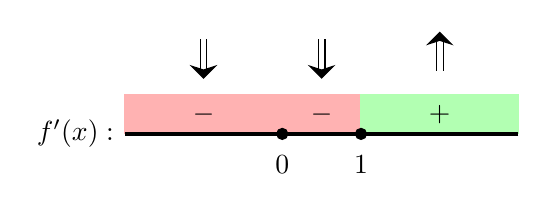
\begin{tikzpicture}[scale=1, baseline]
                            \def\critpoints{0/black, 1/black}
                            \def\maxint{3}
                            \def\minint{-2}
                            \def\plus{+}

                            %===== Naik/Turun =====
                            % Format: titik_awal / titik_akhir / tanda
                            \foreach \start/\end/\sign in {\minint/0/-, 0/1/-, 1/\maxint/+} {

                                    % Logika IF untuk menentukan Warna dan Arah Panah
                                    \ifx\sign\plus
                                        \def\mycolor{green!30}  % Warna Hijau
                                        \def\yArrow{0.8}          % Posisi Y awal panah (bawah)
                                        \def\dyArrow{0.5}       % Arah panah (ke atas)
                                    \else
                                        \def\mycolor{red!30}    % Warna Merah
                                        \def\yArrow{1.2}        % Posisi Y awal panah (atas)
                                        \def\dyArrow{-0.5}      % Arah panah (ke bawah)
                                    \fi

                                    \draw[fill=\mycolor, draw=\mycolor] (\start,0) rectangle (\end,0.5) node[midway,black] {$\sign$};

                                    % 2. Gambar Panah
                                    % Titik tengah x dihitung otomatis: (\start + \end) / 2
                                    \draw[double arrow] ({(\start+\end)/2}, \yArrow) -- ++(0, \dyArrow);
                                }
                            %===== GARIS BILANGAN =====
                            \draw[very thick] (\maxint,0) -- (\minint,0) node[left] {$f'(x):$};
                            % loop titik kritis
                            \foreach \x/\c in \critpoints{
                                \draw[fill=\c] (\x,0) circle (2pt);
                                \node[below] at (\x,-0.15) {$\x$}; % label angka
                            }
                        \end{tikzpicture}
                    \end{center}
                    Dari gambar di atas, diperoleh:
                    \begin{itemize}
                        \item Fungsi turun pada interval \( (-\infty, 0) \cup (0, 1) \).
                        \item Fungsi naik pada interval \( (1, \infty) \).
                    \end{itemize}
              \item Titik ekstrem relatif terjadi pada titik kritis \( f'(x) \), yaitu \( x = 0 \) dan \( x = 1 \). Namun karena \( f'(x) \) tidak berganti tanda di sekitar \( x = 0 \), maka titik tersebut bukan titik ekstrem. Sedangkan pada \( x = 1 \), fungsi berganti dari turun ke naik, sehingga terdapat titik minimum relatif pada \( x = 1 \). Nilai fungsi pada titik tersebut adalah
                    \[
                        f(1) = 3(1)^4 - 8(1)^3 + 6(1)^2 + 1 = 3 - 8 + 6 + 1 = 2.
                    \]
                    Jadi, titik minimum relatifnya adalah \( (1, 2) \).
              \item Untuk menentukan selang kecekungan, maka diperlukan informasi mengenai tanda dari \( f''(x) \).
                    Turunkan \( f'(x) \):
                    \[
                        f''(x) = 36x^2 - 48x + 12 = 12(3x^2 - 4x + 1) = 12(3x - 1)(x - 1).
                    \]
                    Selanjutnya, tinjau tanda \( f''(x) \):
                    \begin{center}
                        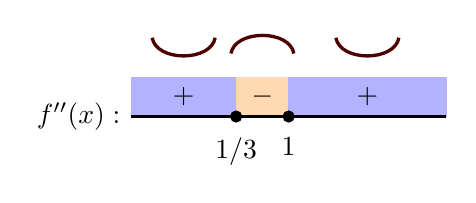
\begin{tikzpicture}[scale=1, baseline]
                            \def\critpoints{1/black, {1/3}/black}
                            \def\maxint{3}
                            \def\minint{-1}
                            \def\plus{+}

                            %===== Naik/Turun =====
                            % Format: titik_awal / titik_akhir / tanda
                            \foreach \start/\end/\sign in {\minint/{1/3}/+, {1/3}/1/-, 1/\maxint/+} {

                            % Logika IF untuk menentukan Warna dan Arah Panah
                            \ifx\sign\plus
                                \def\mycolor{blue!30}
                                \def\dyArc{1}
                                \def\direction{right}
                            \else
                                \def\mycolor{orange!30}
                                \def\dyArc{0.8}
                                \def\direction{left}
                            \fi

                            \draw[fill=\mycolor, draw=\mycolor] ({\start},0) rectangle ({\end},0.5) node[midway,black] {$\sign$};

                            \draw[very thick, black!70!red]
                            ({(\start+\end)/2 - 0.4}, \dyArc)
                            to[bend \direction=80]
                            ({(\start+\end)/2 + 0.4}, \dyArc);
                            }
                            %===== GARIS BILANGAN =====
                            \draw[very thick] (\maxint,0) -- (\minint,0) node[left] {$f''(x):$};
                            % loop titik kritis
                            \foreach \x/\c in \critpoints{
                                \draw[fill=\c] ({\x},0) circle (2pt);
                                \node[below] at ({\x},-0.15) {$\x$}; % label angka
                            }
                        \end{tikzpicture}
                    \end{center}
                    Dari gambar di atas, diperoleh:
                    \begin{itemize}
                        \item Fungsi cekung ke atas pada interval \( (-\infty, \frac{1}{3}) \cup (1, \infty) \).
                        \item Fungsi cekung ke bawah pada interval \( (\frac{1}{3}, 1) \).
                        \item Titik belok terjadi pada titik kritis \( f''(x) \), yaitu \( x = \frac{1}{3} \) dan \( x = 1 \).
                    \end{itemize}
              \item Sketsa grafiknya adalah sebagai berikut:
                    \begin{center}
                        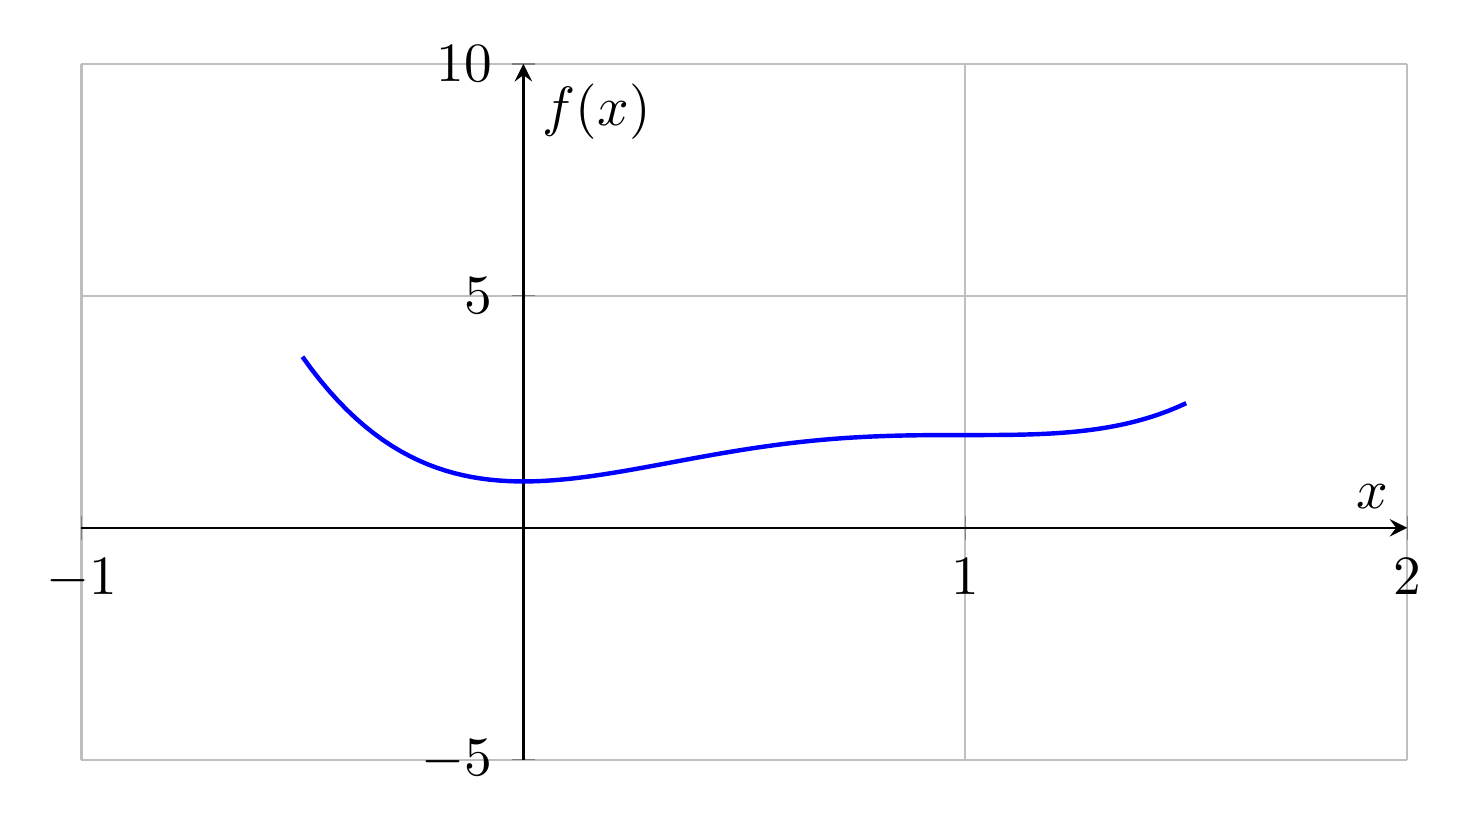
\begin{tikzpicture}[scale=2]
                            \begin{axis}[
                                    axis lines = middle,
                                    xlabel = \(x\),
                                    ylabel = {\(f(x)\)},
                                    xtick={-1,0,1,2},
                                    ytick={-5,0,5,10},
                                    ymin=-5, ymax=10,
                                    xmin=-1, xmax=2,
                                    domain=-0.5:1.5,
                                    samples=100,
                                    grid=both,
                                    width=10cm,
                                    height=6cm
                                ]
                                \addplot[thick,blue] {3*x^4 - 8*x^3 + 6*x^2 + 1};
                            \end{axis}
                        \end{tikzpicture}
                    \end{center}
          \end{enumerate}
    \item ,
    \item ,
\end{enumerate}

\newpage
\renewcommand{\arraystretch}{1}
\fancyhead{}
\fancyfoot{}
\fancyhead[r]{}
\fancyhead[l]{\fbox{\large{\textbf{SKPB - ITS}}}}
\renewcommand{\headrulewidth}{0pt}
\renewcommand{\footrulewidth}{0pt}
\begin{center}
    {\underline{\textbf{\MakeUppercase{Evaluasi Akhir Semester Bersama Ganjil 2024/2025}}}}
\end{center}

\begin{center}
    \begin{tabular}{lcl}
        Mata kuliah/SKS & : & Kalkulus 1 ( SM234101 ) / 3 SKS \\
        Hari, Tanggal   & : & Kamis, 12 Desember 2024         \\
        Waktu           & : & 13.30-15.10 WIB (100 menit)     \\
        Sifat           & : & Tertutup                        \\
        Kelas           & : & 34-46, 107, 108
    \end{tabular}
\end{center}

\noindent\rule{\textwidth}{2.pt}

\setlength{\parindent}{5pt}
\setlength{\parindent}{5pt}
\centering{Tuliskan: Nama, NRP, dan Nomor Kelas pada lembar jawaban Anda.}
\setlength{\parindent}{5pt}
\par \textbf{\small\MakeUppercase{dilarang membawa/menggunakan kalkulator dan alat komunikasi}}
\centering{\textbf{\MakeUppercase{dilarang memberikan/menerima jawaban selama ujian}}}
\par \centering{\textbf{"Setiap tindak kecurangan akan mendapat sanksi akademik."}}
\noindent\rule{\textwidth}{2.pt}

\begin{table}[h]
    \centering
    EAS Mengukur Kemampuan
    \begin{tabular}{|c|m{10.5cm}|c|c|}
        \hline
        CPL & CPMK                                                                                                          & SOAL & BOBOT (\%) \\ \hline
        \multirow{5}{*}{2}
            & CPMK-2 Mampu menentukan kekontinuan fungsi dan                                                                & 1    & 20         \\ \cline{3-4}
            & turunannya                                                                                                    & 2    & 20         \\\cline{2-4}
            & CPMK-3 Mampu menghitung integral melalui teorema fundamental kalkulus                                         & 3    & 20         \\ \cline{2-4}
            & CPMK-4 Mampu mengaplikasikan bentuk peubah kompleks dalam bentuk polar serta mencari akar-akar persamaannya   & 4    & 20         \\ \cline{2-4}
            & CPMK-5 Mampu menerapkan konsep matriks untuk menyelesaikan sistem persamaan linier dan menentukan nilai eigen & 5    & 20         \\ \hline
    \end{tabular}
\end{table}
{\centering\textbf{SOAL}}
% SOAL DI SINI YAA
\begin{enumerate}
    \item Diberikan kurva $y = \sqrt{x}$ untuk $0 \leq x \leq 3$. Dapatkan titik pada kurva yang memiliki jarak terdekat dengan titik $(2, 0)$.

    \item Diberikan fungsi $f(x) = \displaystyle\frac{x}{x - 2024}$.
          \begin{enumerate}
              \item Tentukan asimtot datar dan tegaknya (jika ada).
              \item Tentukan selang dimana fungsi $f(x)$ naik atau turun.
              \item Tentukan titik ekstrim relatif fungsi tersebut.
              \item Tentukan selang kecekungan fungsi $f(x)$ dan titik belok (jika ada).
              \item Sketsa grafiknya.
          \end{enumerate}

    \item Misalkan $F(x) = \displaystyle\int_{-1}^x \frac{1 + t^3}{1 + t^2} \, dt$. Dapatkan $F(-1)$, $F'(-1)$, dan $F''(-1)$.

    \item Nyatakan bilangan kompleks $\displaystyle z = \left(\frac{\left(1 + i\right)^{12}\left(1 + i\sqrt{3}\right)^{16}}{(-1 + i)^{32}}\right)$ dalam bentuk $z = a + bi$.

    \item Carilah nilai $x_3$ dari sistem persamaan linear berikut:
          \begin{align*}
              x_1 + 4x_3 + x_4        & = 11, \\
              2x_1 + 3x_3 + 2x_4      & = 12, \\
              5x_1 + x_2 + 2x_3 + x_4 & = 20, \\
              4x_1 + 6x_3 + x_4       & = 24,
          \end{align*}
          dengan menggunakan metode Cramer.
\end{enumerate}
\fancyfoot{\begin{center}
        \rule{0.28\textwidth}{2.pt}$\quad$\textbf{Selamat Mengerjakan}$\quad$\rule{0.28\textwidth}{2.pt}
        \begin{quote}
            \centering
            \textit{``Jujur adalah kunci kesuksesan''}
        \end{quote}
    \end{center}}

\newpage
\fancyhead[L]{\textit{Solution By: \hyperlink{https://github.com/TetewHeroez}{Tetew}}}
\fancyfoot{}
% \fancyfoot[R]{\animategraphics[autoplay,loop,width=0.1\textwidth]{15}{Kuru Kuru Herta/kuru kuru-}{0}{5}}
{\centering\textbf{SOLUSI}}
\renewcommand{\arraystretch}{1.5}
\renewcommand{\headrulewidth}{1pt}
\begin{enumerate}
    \item Pertama-tama dari soal kita tahu bahwa titik yang berada pada kurva memiliki koordinat $(x, \sqrt{x})$. Kemudian jarak antara titik $(x, \sqrt{x})$ dengan titik $(2, 0)$ dapat didefinsikan dengan
          \[D(x)= \sqrt{(x-2)^2 + (\sqrt{x} - 0)^2} = \sqrt{x^2 - 4x + 4 + x} = \sqrt{x^2 - 3x + 4}.\]
          Dapat dilihat bahwa $D(x)$ merupakan fungsi yang bergantung pada $x$ dengan interval $0 \leq x \leq 3$. Untuk mencari nilai minimum dari $D(x)$, kita cari titik stasioner dari $D(x)$ dengan mencari turunan pertama dari $D(x)$, yaitu
          \[D'(x) = \frac{2x - 3}{2\sqrt{x^2 - 3x + 4}} = 0 \implies x = \frac{3}{2}.\]
          Karena kita bekerja pada interval yang terbatas, maka kita juga perlu mengecek nilai $D(x)$ pada titik-titik ujung interval, sehingga dapat dibandingkan nilainya pada tabal dibawah ini
          \begin{center}
              \begin{tabular}{|c|c|c|c|}
                  \hline
                  $x$    & $0$ & $3/2$ & $3$ \\ \hline
                  $D(x)$ & $2$ & $7/4$ & $2$ \\ \hline
              \end{tabular}
          \end{center}
          Sehingga titik yang memiliki jarak terdekat dengan titik $(2, 0)$ adalah ketika $x = 3/2$. Yang terakhir subtitusikan nilai $x = 3/2$ ke dalam $y = \sqrt{x}$.\\

          $\therefore$ Titik yang memiliki jarak terdekat dengan titik $(2, 0)$ adalah $\left(\displaystyle\frac{3}{2}, \sqrt{\frac{3}{2}}\right)$.

    \item KIta dapat rubah fungsi $f(x)$ agar lebih sederhana saat diturunkan
          \[f(x) = \frac{x}{x - 2024} = \frac{(x-2024)+2024}{x-2024}=1+\frac{2024}{x-2024}\]
          \begin{enumerate}
              \item Asimtot datar terjadi ketika $f(x)$ mendekati nilai konstan ketika $x$ mendekati $\pm \infty$.
                    \[\lim_{x \to \infty} f(x) = \lim_{x \to \infty} 1+\frac{2024}{x-2024} = 1\]
                    $\therefore$ Asimtot datar terjadi pada $y = 1$. \\~\\

                    Asimtot tegak terjadi ketika $f(x)$ mendekati nilai tak hingga ketika $x$ mendekati suatu nilai tertentu. Dalam hal ini, asimtot tegak terjadi ketika penyebut dari $f(x)$ adalah nol, yaitu ketika $x = 2024$.
              \item Tinjau turunan pertama dari $f(x)$
                    \begin{align*}
                        f'(x) & = \frac{d}{dx}\left(1+\frac{2024}{x-2024}\right) = \frac{d}{dx}\left(\frac{x-2024+2024}{x-2024}\right)                     \\
                              & = \frac{d}{dx}\left(1+\frac{2024}{x-2024}\right) = \frac{d}{dx}\left(\frac{2024}{x-2024}\right) = -\frac{2024}{(x-2024)^2}
                    \end{align*}
                    Karena $f'(x)\neq 0$ untuk semua $x\in\R$, maka titik kritis dari $f(x)$ hanya terjadi ketika $x=2024$.\\
                    Uji titik:
                    \begin{itemize}
                        \item $x = 0 \implies f'(0) = -\frac{1}{2024} < 0$.
                        \item $x = 2025 \implies f'(2025) = -2024 < 0$.
                    \end{itemize}
                    \begin{center}
                        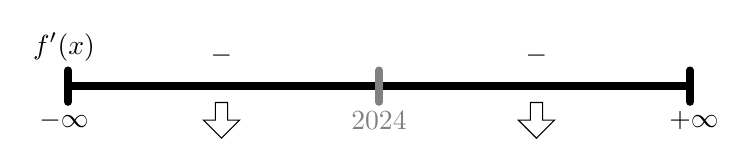
\begin{tikzpicture}[
                                every node/.style = {minimum size=1em,inner sep=2pt},
                                Arrow/.style = {single arrow, draw, minimum height=3ex,
                                        single arrow head extend=1ex,
                                        shape border rotate=#1}
                            ]
                            \draw[line width=1mm,{Bar[width=4mm,round]}-{Bar[width=4mm,round]}]
                            (0,0) node [above=2mm] {$f'(x)$}
                            node [below=2mm] {$-\infty$}  -- ++
                            (8,0) node [above=2mm] {}
                            node [below=2mm] {$+\infty$} ;
                            \draw[line width=1mm,line cap=round,gray]
                            (4,-0.2) node[below] {$2024$} -- ++ (0,0.4);
                            % signs    
                            \node[above] at (2,0.2) {$-$};
                            \node[above] at (6,0.2) {$-$};
                            % arrows
                            \node[Arrow= 270, below] at (2,-0.2) {};
                            \node[Arrow= 270, below] at (6,-0.2) {};
                        \end{tikzpicture}
                    \end{center}
                    $\therefore$ Fungsi $f(x)$ selalu turun pada selang $(-\infty, 2024)\cup(2024, +\infty)$.
              \item Karena $f'(x)$ tidak akan pernah nol, maka fungsi $f(x)$ tidak memiliki titik ekstrim.
              \item Tinjau turunan kedua dari $f(x)$
                    \begin{align*}
                        f''(x) & = \frac{d}{dx}\left(-\frac{2024}{(x-2024)^2}\right) = \frac{4048}{(x-2024)^3}
                    \end{align*}
                    Karena $f''(x) \neq 0$ untuk semua $x\in\R$, maka fungsi $f(x)$ tidak memiliki titik belok.\\
                    Uji titik:
                    \begin{itemize}
                        \item $x = 0 \implies f''(0) = -\frac{2}{2024^2} < 0$.
                        \item $x = 2025 \implies f''(2025) =  4048> 0$.
                    \end{itemize}
                    \begin{center}
                        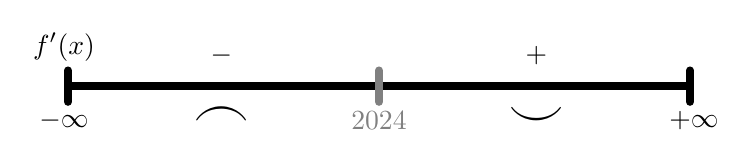
\begin{tikzpicture}[
                                every node/.style = {minimum size=1em,inner sep=2pt},
                                Arrow/.style = {single arrow, draw, minimum height=3ex,
                                        single arrow head extend=1ex,
                                        shape border rotate=#1}
                            ]
                            \draw[line width=1mm,{Bar[width=4mm,round]}-{Bar[width=4mm,round]}]
                            (0,0) node [above=2mm] {$f'(x)$}
                            node [below=2mm] {$-\infty$}  -- ++
                            (8,0) node [above=2mm] {}
                            node [below=2mm] {$+\infty$} ;
                            \draw[line width=1mm,line cap=round,gray]
                            (4,-0.2) node[below] {$2024$} -- ++ (0,0.4);
                            % signs    
                            \node[above] at (2,0.2) {$-$};
                            \node[above] at (6,0.2) {$+$};
                            % arrows
                            \node[below] at (2,-0.2) {\huge$\frown$};
                            \node[below] at (6,-0.2) {\huge$\smile$};
                        \end{tikzpicture}
                    \end{center}
                    $\therefore$ Fungsi $f(x)$ cekung ke bawah pada selang $(-\infty, 2024)$ dan cekung ke atas pada selang $(2024, +\infty)$.
              \item Dapat kita sketsa menggunakan informasi pergeseran grafik dari $f(x)=\dfrac{1}{x}$. (2024 satuan ke kanan dan 1 satuan ke atas)
                    \begin{center}
                        \begin{tikzpicture}[scale=0.8]
                            \draw [->] (-2,0) -- (7,0) node [right] {\footnotesize$x$};
                            \draw [->] (0,-2) -- (0,4) node [above] {\footnotesize$y$};

                            \draw [domain=4:7, samples=50, thick, blue] plot (\x, {\x/(\x-3)});
                            \draw [domain=-2:2, samples=50, thick, blue] plot (\x, {\x/(\x-3)});
                            \draw [domain=-2:4, samples=10, darkgray, dashed] plot (3, {\x});
                            \draw [domain=-2:7, samples=10, darkgray, dashed] plot ({\x}, 1);

                            \node [below right] at (3,0) {\footnotesize$2024$};
                            \node [below right] at (0,1) {\footnotesize$1$};
                        \end{tikzpicture}
                    \end{center}
          \end{enumerate}
    \item Untuk $F(-1)$, dapat dilihat karena nilai batas bawah dan batas atas sama, maka nilai integralnya adalah nol.
          \begin{flalign*}
              F(-1) & = \int_{-1}^{-1} \frac{1 + t^3}{1 + t^2} \, dt = 0 &
          \end{flalign*}
          Selanjutnya untuk $F'(-1)$, dapat kita gunakan Teorema Fundamental Kalkulus II untuk mencari turunan dari $F(x)$.
          \begin{flalign*}
              F'(x)  & = \frac{d}{dx}\left(\int_{-1}^x \frac{1 + t^3}{1 + t^2} \, dt\right) = \frac{1 + x^3}{1 + x^2} & \\
              F'(-1) & = \frac{1 + (-1)^3}{1 + (-1)^2} = 0                                                            &
          \end{flalign*}
          Terakhir untuk $F''(-1)$, kita turunkan $F'(x)$.
          \begin{flalign*}
              F''(x)  & = \frac{d}{dx}\left(\frac{1 + x^3}{1 + x^2}\right) = \frac{3x^2(1 + x^2) - 2x(1 + x^3)}{(1 + x^2)^2} & \\
              F''(-1) & = \frac{3(-1)^2(1 + (-1)^2) - 2(-1)(1 + (-1)^3)}{(1 + (-1)^2)^2} = \frac{3(2)-0}{4}=\frac{3}{2}      &
          \end{flalign*}

    \item Agar lebih mudah dihitung, jadikan ketiga masing-masing bilangan kompleks diatas menjadi bentuk polar.
          \begin{itemize}
              \item Untuk $1+i$, didapatkan $a=1$ dan $b=1$ sehingga $r=\sqrt{1^2+1^2}=\sqrt{2}$ dan $\theta=\arctan\left(1\right)=\dfrac{\pi}{4}$ (Kuadran I).\footnote{Boleh dijadikan dalam bentuk derajat}
              \item Untuk $1+i\sqrt{3}$, didapatkan $a=1$ dan $b=\sqrt{3}$ sehingga $r=\sqrt{1^2+(\sqrt{3})^2}=2$ dan $\theta=\arctan\left(\sqrt{3}\right)=\dfrac{\pi}{3}$ (Kuadran I).
              \item Untuk $-1+i$, didapatkan $a=-1$ dan $b=1$ sehingga $r=\sqrt{(-1)^2+1^2}=\sqrt{2}$ dan $\theta=\arctan\left(-1\right)=\dfrac{3\pi}{4}$ (Kuadran II).
          \end{itemize}
          Jadi bentuk polar dari $z$ adalah
          \begin{align*}
              z & =\left(\frac{\left(1 + i\right)^{12}\left(1 + i\sqrt{3}\right)^{16}}{(-1 + i)^{32}}\right)=\frac{\left[\sqrt{2}\cis\left(\dfrac{\pi}{4}\right)\right]^{12}\left[2\cis\left(\dfrac{\pi}{3}\right)\right]^{16}}{\left[\sqrt{2}\cis\left(\dfrac{3\pi}{4}\right)\right]^{32}}=\frac{\left[2^{6}\cis\left(3\pi\right)\right]\left[\cancel{2^{16}}\cis\left(\dfrac{16\pi}{3}\right)\right]}{\cancel{2^{16}}\cis\left(24\pi\right)} \\
                & =\frac{\left[2^{6}\cis\left(\pi\right)\right]\left[\cis\left(\dfrac{4\pi}{3}\right)\right]}{\cis\left(0\right)}=2^{6}\cis\left(\pi+\dfrac{4\pi}{3}-0\right)=2^{6}\cis\left(\dfrac{7\pi}{3}\right)=2^{6}\cis\left(\dfrac{\pi}{3}\right)                                                                                                                                                                                       \\
                & =64\left(\cos\left(\dfrac{\pi}{3}\right)+i\sin\left(\dfrac{\pi}{3}\right)\right)=64\left(\dfrac{1}{2}+i\dfrac{\sqrt{3}}{2}\right)=\boxed{32+32\sqrt{3}i}
          \end{align*}
    \item Metode Cramer secara umum untuk mencari nilai $x_n$ dapat dirumuskan sebagai
          \[x_n=\frac{\det(A_n)}{\det(A)}\]
          dengan $A_n$ adalah matriks yang diperoleh dari matriks $A$ yang kolom ke-$n$-nya diganti dengan vektor kolom $b$. (Dalam hal ini $n=3$)

          SPL diatas dapat dituliskan dalam bentuk matriks sebagai berikut
          \[\underbrace{\begin{pmatrix}
                      1 & 0 & 4 & 1 \\
                      2 & 0 & 3 & 2 \\
                      5 & 1 & 2 & 1 \\
                      4 & 0 & 6 & 1
                  \end{pmatrix}}_{A}\underbrace{\begin{pmatrix}
                      x_1 \\x_2\\x_3\\x_4
                  \end{pmatrix}}_{x}=\underbrace{\begin{pmatrix}
                      11 \\12\\20\\24
                  \end{pmatrix}}_{b}\]
          Kemudian kita tulis matriks $A_3$ dengan mengganti kolom ke-3 dari matriks $A$ dengan vektor kolom $b$.
          \[A_3=\begin{pmatrix}
                  1 & 0 & 11 & 1 \\
                  2 & 0 & 12 & 2 \\
                  5 & 1 & 20 & 1 \\
                  4 & 0 & 24 & 1
              \end{pmatrix}\]
          Selanjutnya kita hitung nilai determinan dari matriks $A$ dan $A_3$. Ada banyak metode untuk menghitung determinan, seperti OBE, ekspansi kofaktor, dsb. Disini saya akan menggunakan metode ekspansi kofaktor dan OBE.\footnote{OBE dan ekspansi kofaktor memang bisa di-\textit{combine} untuk mempercepat perhitungan}
          \begin{itemize}
              \item Untuk $\det(A)$, pertama akan kita ekspansi kofaktor sepanjang kolom kedua karena memiliki banyak nol.
                    \begin{align*}
                        \begin{vmatrix}
                            1 & 0 & 4 & 1 \\
                            2 & 0 & 3 & 2 \\
                            5 & 1 & 2 & 1 \\
                            4 & 0 & 6 & 1
                        \end{vmatrix}=-0...+0...-(1)\begin{vmatrix}
                                                        1 & 4 & 1 \\
                                                        2 & 3 & 2 \\
                                                        4 & 6 & 1
                                                    \end{vmatrix}+0...=-\begin{vmatrix}
                                                                            1 & 4 & 1 \\
                                                                            2 & 3 & 2 \\
                                                                            4 & 6 & 1
                                                                        \end{vmatrix}
                    \end{align*}
                    Untuk matrix $3\times 3$ kita bisa menggunakan aturan Sarrus, namun disini saya akan menggunakan OBE yaitu $B_2-2B_1$ dan $B_3-4B_1$.\footnote{OBE tipe ini tidak mengubah nilai determinan matriks awal}
                    \begin{align*}
                        -\begin{vmatrix}
                             1 & 4 & 1 \\
                             2 & 3 & 2 \\
                             4 & 6 & 1
                         \end{vmatrix} & =-\begin{vmatrix}
                                               1 & 4   & 1  \\
                                               0 & -5  & 0  \\
                                               0 & -10 & -3
                                           \end{vmatrix}=-\begin{vmatrix}
                                                              -5  & 0  \\
                                                              -10 & -3
                                                          \end{vmatrix}=-[(-5)(-3)-(-10)0]=-15
                    \end{align*}
              \item Untuk $\det(A_3)$, dengan langkah yang sama kita ekspansi kofaktor sepanjang kolom kedua.
                    \begin{align*}
                        \begin{vmatrix}
                            1 & 0 & 11 & 1 \\
                            2 & 0 & 12 & 2 \\
                            5 & 1 & 20 & 1 \\
                            4 & 0 & 24 & 1
                        \end{vmatrix}=-0...+0...-(1)\begin{vmatrix}
                                                        1 & 11 & 1 \\
                                                        2 & 12 & 2 \\
                                                        4 & 24 & 1
                                                    \end{vmatrix}+0...=-\begin{vmatrix}
                                                                            1 & 11 & 1 \\
                                                                            2 & 12 & 2 \\
                                                                            4 & 24 & 1
                                                                        \end{vmatrix}
                    \end{align*}
                    Dan kita gunakan OBE yang sama yaitu $B_2-2B_1$ dan $B_3-4B_1$.
                    \begin{align*}
                        -\begin{vmatrix}
                             1 & 11 & 1 \\
                             2 & 12 & 2 \\
                             4 & 24 & 1
                         \end{vmatrix} & =-\begin{vmatrix}
                                               1 & 11  & 1  \\
                                               0 & -10 & 0  \\
                                               0 & -20 & -3
                                           \end{vmatrix}=-\begin{vmatrix}
                                                              -10 & 0  \\
                                                              -20 & -3
                                                          \end{vmatrix}=-[(-10)(-3)-(-20)0]=-30
                    \end{align*}
          \end{itemize}
          Terakhir kita gunakan rumus Cramer untuk mencari nilai $x_3$.
          \[x_3=\frac{\det(A_3)}{\det(A)}=\frac{-30}{-15}=2\]
\end{enumerate}
\end{document}